\chapter{Event selection and particle identification}
\label{analysis}
This chapter discusses the selection of events based on their relevance for this thesis. At the beginning of this chapter, the conversion of signal to actual data files is discussed. Following, the event selection and individual cuts will be explained and reasoned. Last section of this chapter debates the conditions imposed on identifying particles. 
\section{Data sample}
\label{data}
Signals, that are measured by the detectors, are moved to Data Acquisition system (DAQ) to be processed. This involves readout and digitization which is facilitated by a Gigalink with the speed of 80 Mb/event, pedestal subtraction, creation of events and lastly moving the data to RHIC Computing Facility (RCF). The transfer is accommodated through a Gigabit ethernet with the speed of 100 Mb/s \cite{DAQ}. Files are saved in the MuDst (MicroDST) format. Essentially, MuDst are ROOT files\cite{ROOT} which include a tree with branches that contain all the information about the events. MuDst files are incredibly large files which contain information and data which is often redundant. That is why a different format is used: PicoDst. PicoDst involves all the necessary data needed and is much more practical. The official framework that has the PicoDst format and involves data from Roman Pot system is called \textit{star-upcDst}.  
\newline
Data taking for this analysis was part of Run17 which happened in 2017. The collisions were proton-proton at center of mass energy $\sqrt{s}=510$ GeV. The analysis was done using the ROOT framework developed by CERN for analysing large data files. The analysis was computated using the RHIC Computing Facility.


\section{Event selection}
This section discusses all the different conditions imposed on measured events to separate the relevant ones. At the beginning, the data set involves $2.03\cdot10^9$ events. \autoref{af1} shows the different cuts and the progress in number of events selected. Different graphs are provided for the different conditions throughout the section. First part explains the Central Production Trigger, then the conditions regarding the forward scattered protons and in the end the hadrons produced in the central system. The distributions shown in this section include data that passed the condition before and show the representation of cuts in black dashed line.

\FloatBarrier
\begin{figure}[ht]
    \centering
    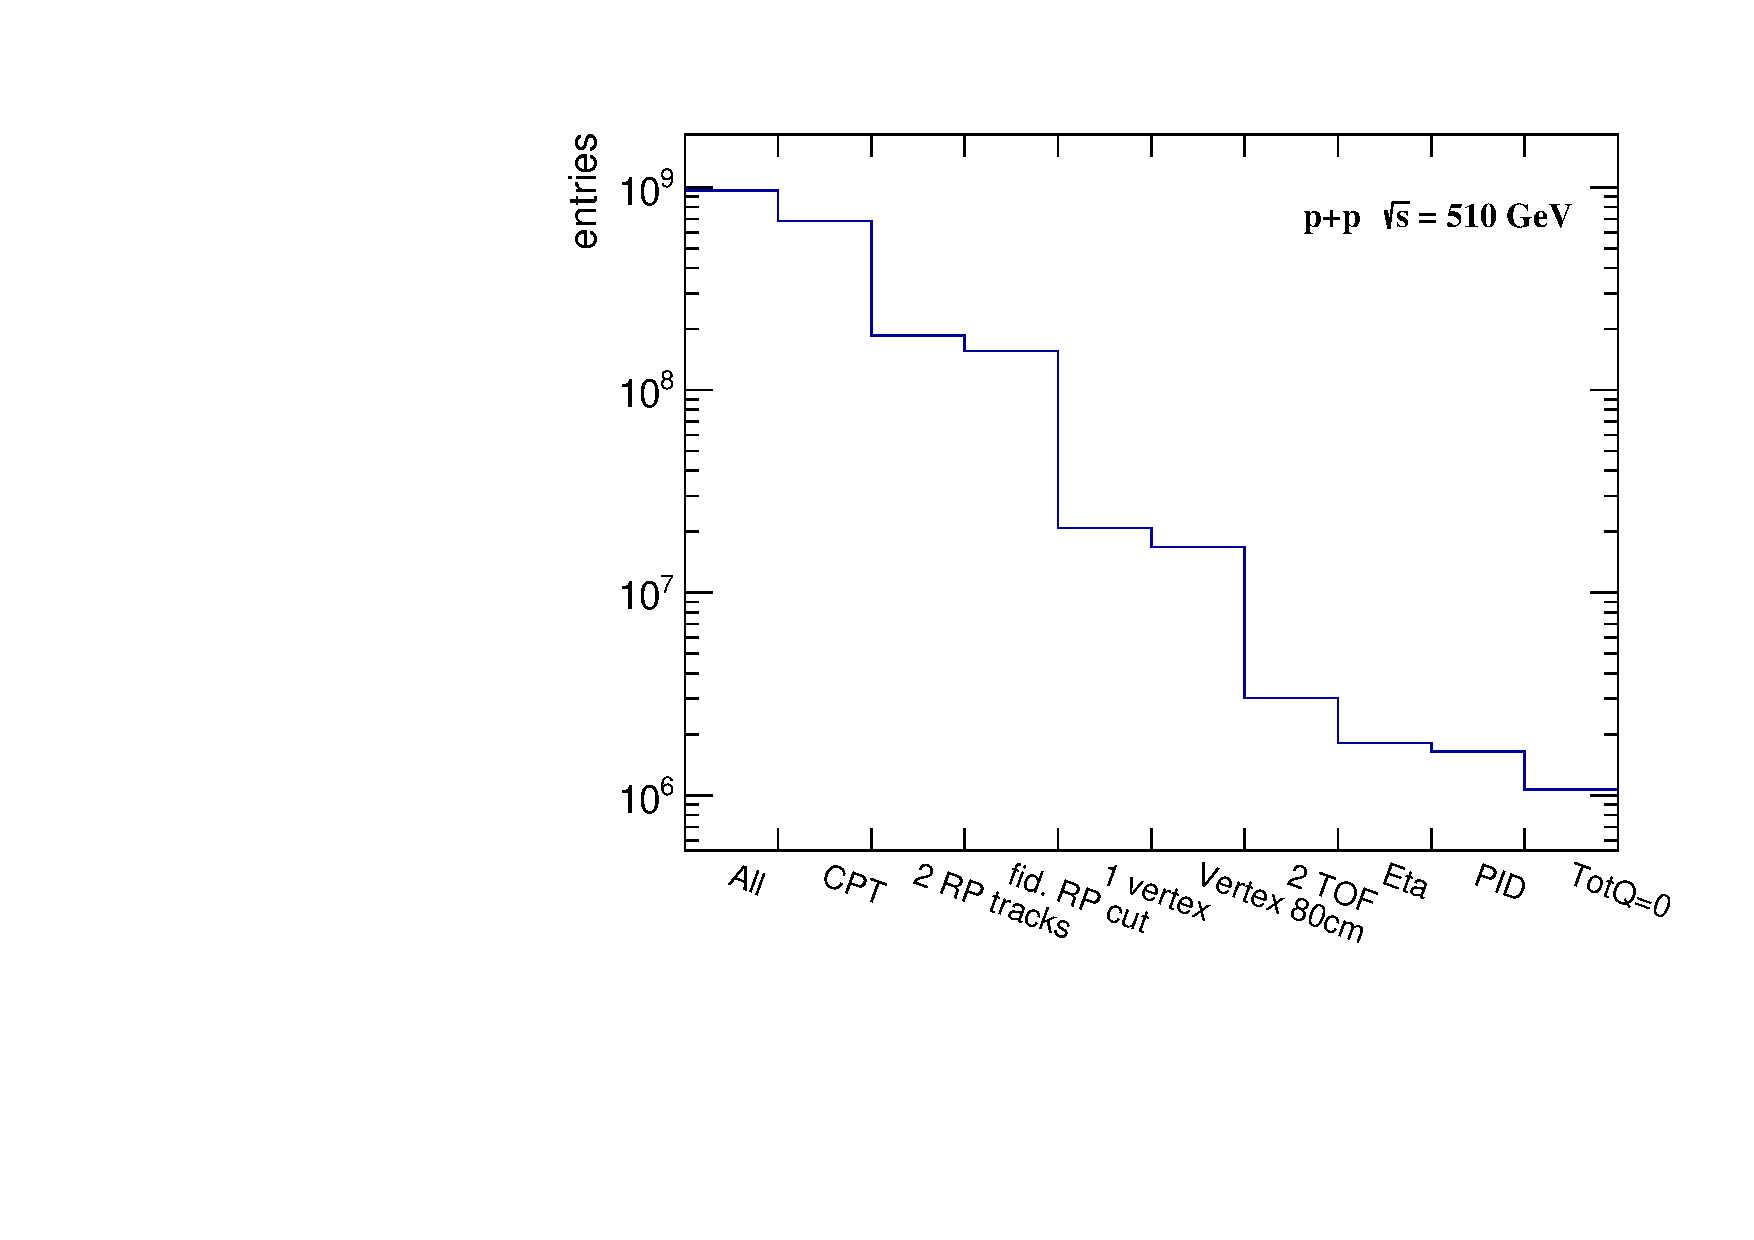
\includegraphics[width=1\textwidth]{figures/AnalysisFlow.pdf}
    \caption[Event selection for production of $K^0_S$ and $\lambda^0$]{Histogram of number of events that pass different cuts.}
    \label{af1}
\end{figure}
\FloatBarrier

\subsection{Central Production Trigger}

\FloatBarrier
\begin{table}[ht]
    \centering
    \begin{tabular}{c|c|c}
    
        condition &  & \\ \hline
       Elastic combination of hits in RP & - & + \\ 
       Inelastic combination of hits in RP & + & - \\
       Number of hits in TOF >1 & + & + \\
       Number of hits in TOF <10 & - & - \\
       Hit in BBC east & - & - \\
       Hit in BBC west & - & - \\
       Hit in BBC Large east & - & -\\
       Hit in BBC Large west & - & - \\
       Hit in ZDC east & - & -\\
       Hit in ZDC west & - & - \\
    \end{tabular}
    \caption[Table of conditions for Central Production Trigger]{Table of conditions Central Production Trigger is comprised of.}
    \label{at38}
\end{table}
\FloatBarrier
The first cut on events is provided by the Central Production Trigger (CPT). All the different conditions this cut involves are listed in \autoref{at38}. First 2 conditions are regarding combinations of hits in Roman Pots. Elastic combination means one proton on each side but one is Up and one is Down. Inelastic combination means on both sides Up or both Down as was discussed in \autoref{STAR}, \autoref{RPs}. Next 2 conditions require  multiplicity in Time Of Flight detector to be between 2 and 10. The rest of the conditions listed regard detectors BBC and ZDC. Beam Beam Counters cover pseudorapidity regions of $3.3<\eta<5$ and Zero Degree Calorimeters are located behind dipole magnets at level of interaction point. The reason for these conditions is to ensure large gaps in rapidity on each side which are distinctive features of diffractive events.
\subsection{2 Roman Pot tracks}

\FloatBarrier
\begin{figure}[ht]
    \centering
    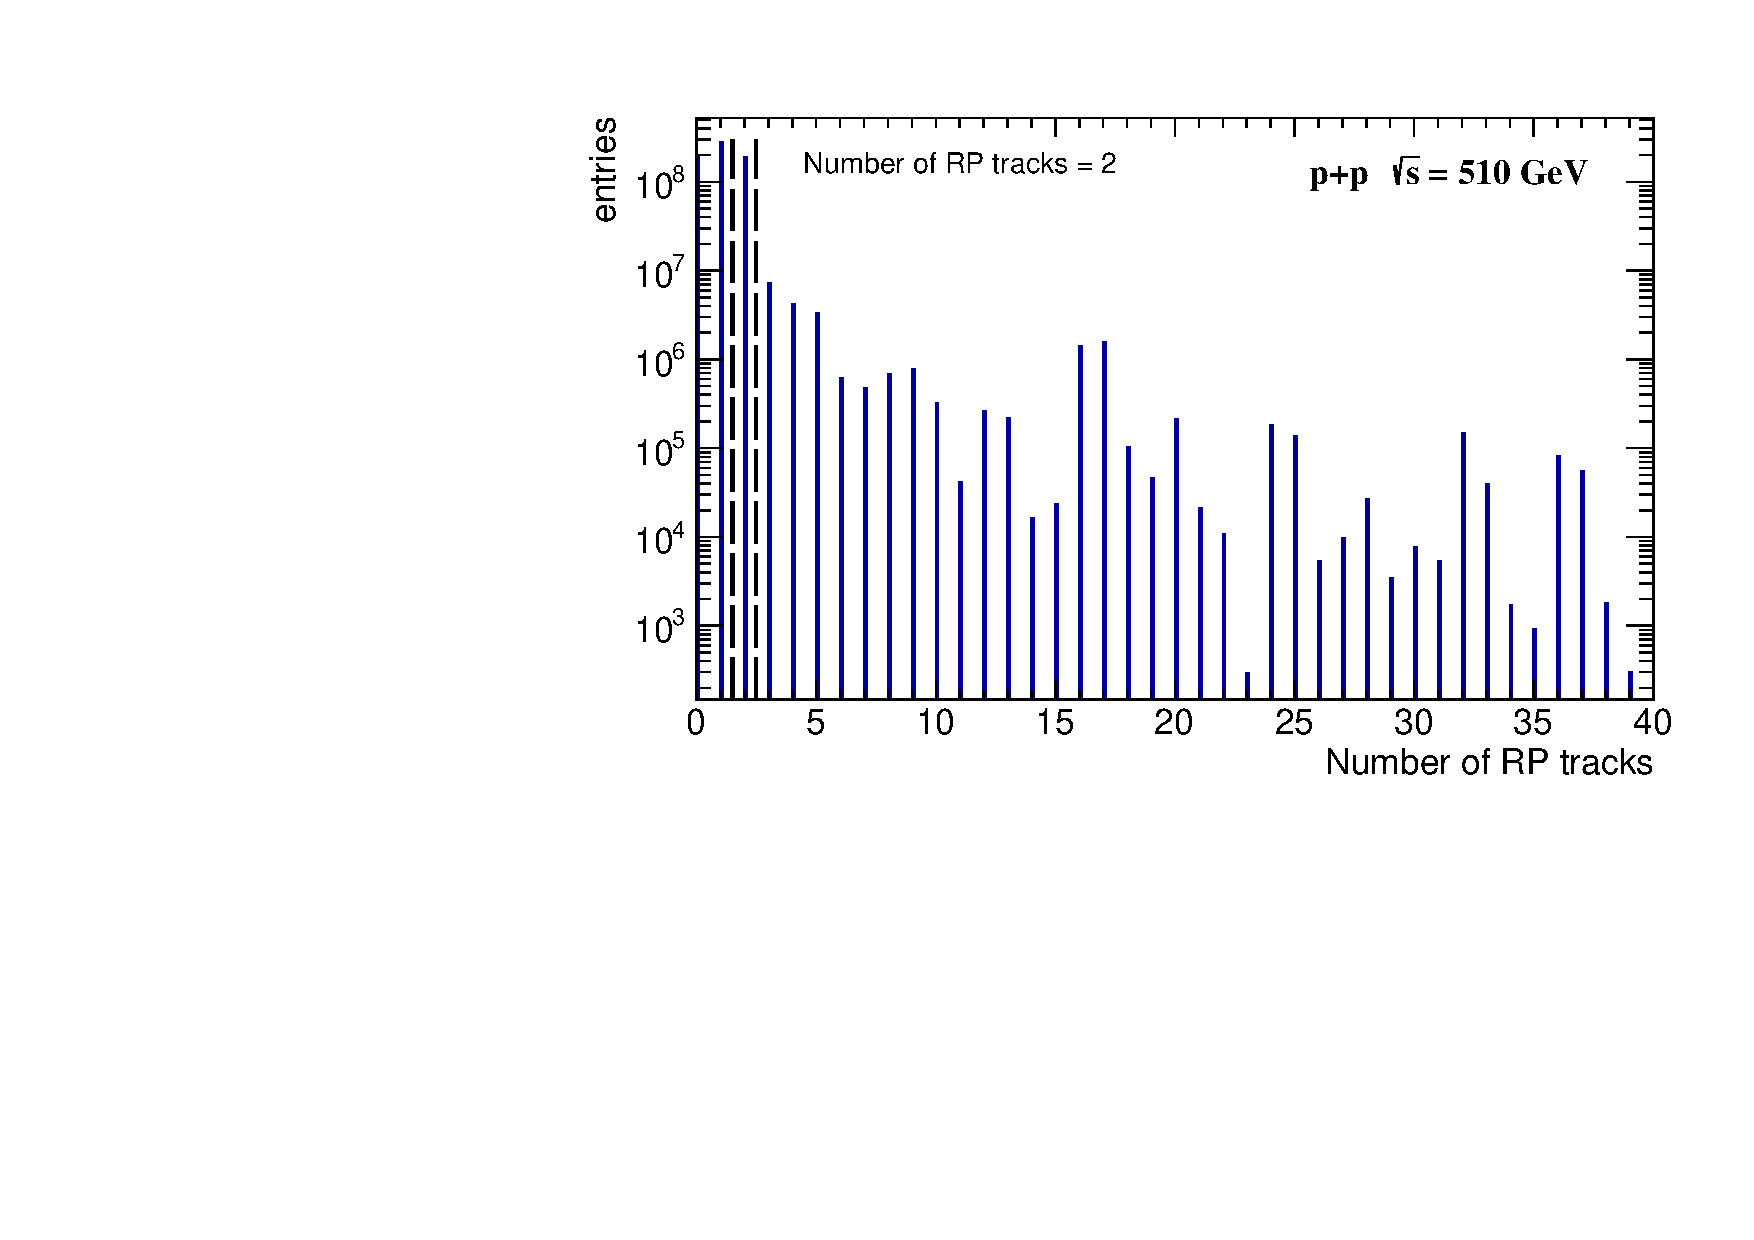
\includegraphics[width=1\textwidth]{figures/NumberRPTracks.pdf}
    \caption[Distribution of number of tracks in Roman Pot system]{Distribution of number of tracks in Roman Pots. The only allowed number is one on the west and one on the east side of the detector.}
    \label{af2}
\end{figure}
\FloatBarrier
The second condition for event selection is that for each event, 2 proton tracks must be registered. Their positions are also important. One track has to be on each side (east or west) of the detector as can be seen in \autoref{df6}. Part of this condition is also the necessity that 3 out of 4 Silicon Strip Detectors inside a Roman Pot have to register a particle. This ensures a certain level accuracy for momentum measurement. The histogram of number of RP tracks per event can be seen in \autoref{af2}. 
\subsection{Fiducial Roman Pot cut}
This next cut focuses on the position of forward protons in transverse plane detected in Roman Pots. To ensure good quality of reconstruction of proton momentum, all the SSD detectors in RPs, that registered a proton, are involved. The fiducial region is estimated to have high geometric acceptance, track reconstruction efficiency and it minimizes the systematic uncertainties\cite{Truhlar}. The fiducial region is defined by the following conditions.
\begin{gather*}  
(p_x + 0.6~\textrm{GeV})^2 + p_y^2 < 1.25 \textrm{ GeV}^2\textrm{/c}^2 \\
0.4 \textrm{ GeV/c } < |p_y| < 0.8 \textrm{ GeV/c} \\
p_x > -0.27 \textrm{ GeV/c}
\label{ea1}
\end{gather*}
\FloatBarrier
\begin{figure}[ht]
    \centering
    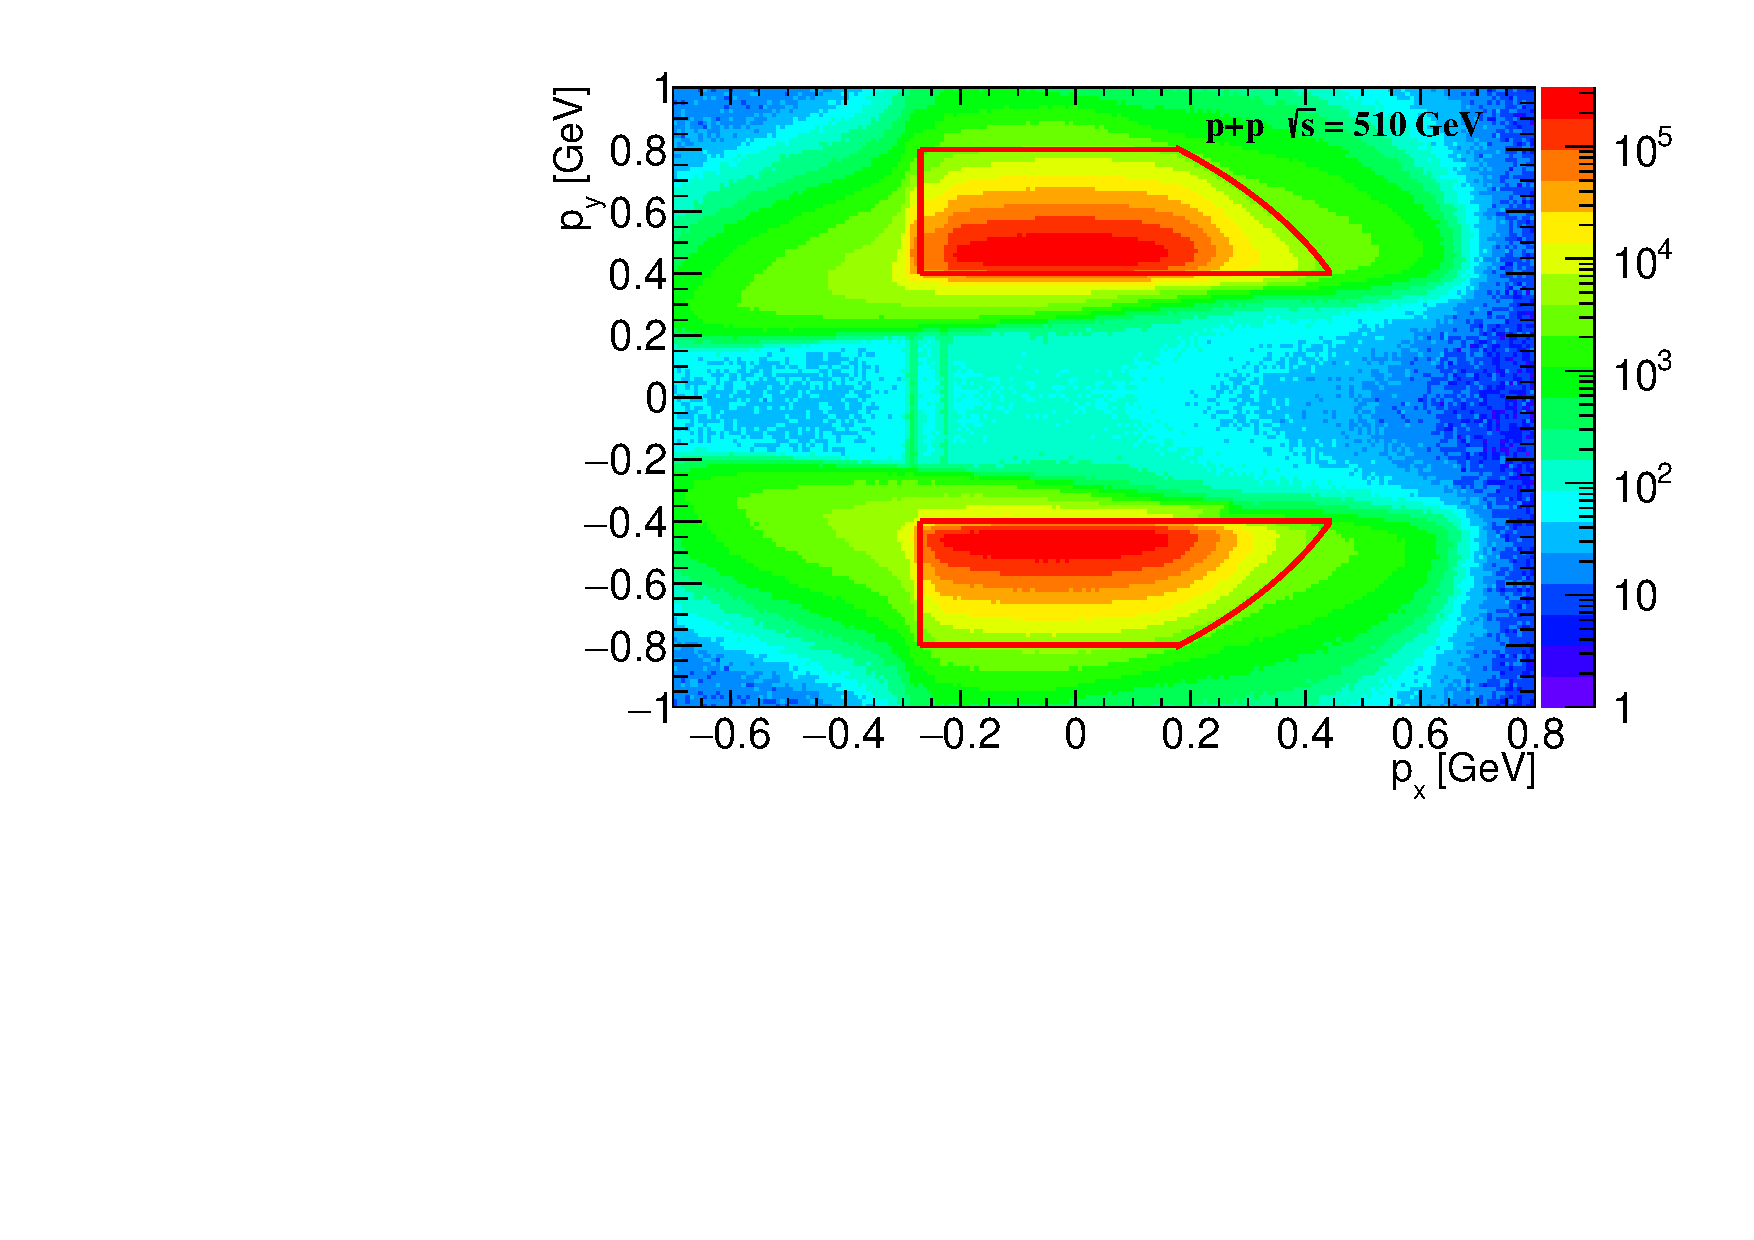
\includegraphics[width=1\textwidth]{figures/hRPcorr.pdf}
    \caption[Correlation graph of transverse momentum in Roman Pot system]{Correlation graph of transverse momenta of scattered protons. Red lines define the fiducial region in Roman Pots.}
    \label{af3}
\end{figure}
\FloatBarrier
The following 2 graphs show the same data but only they are differentiated based on the side where they were measured. Graphs do show a slight shift between the lines that represent the fiducial cut and the position of the structure in the middle. This shift is caused by the displacement of the detectors on the east side by 3 mm. 

\FloatBarrier
\begin{figure}[ht]
    \centering
    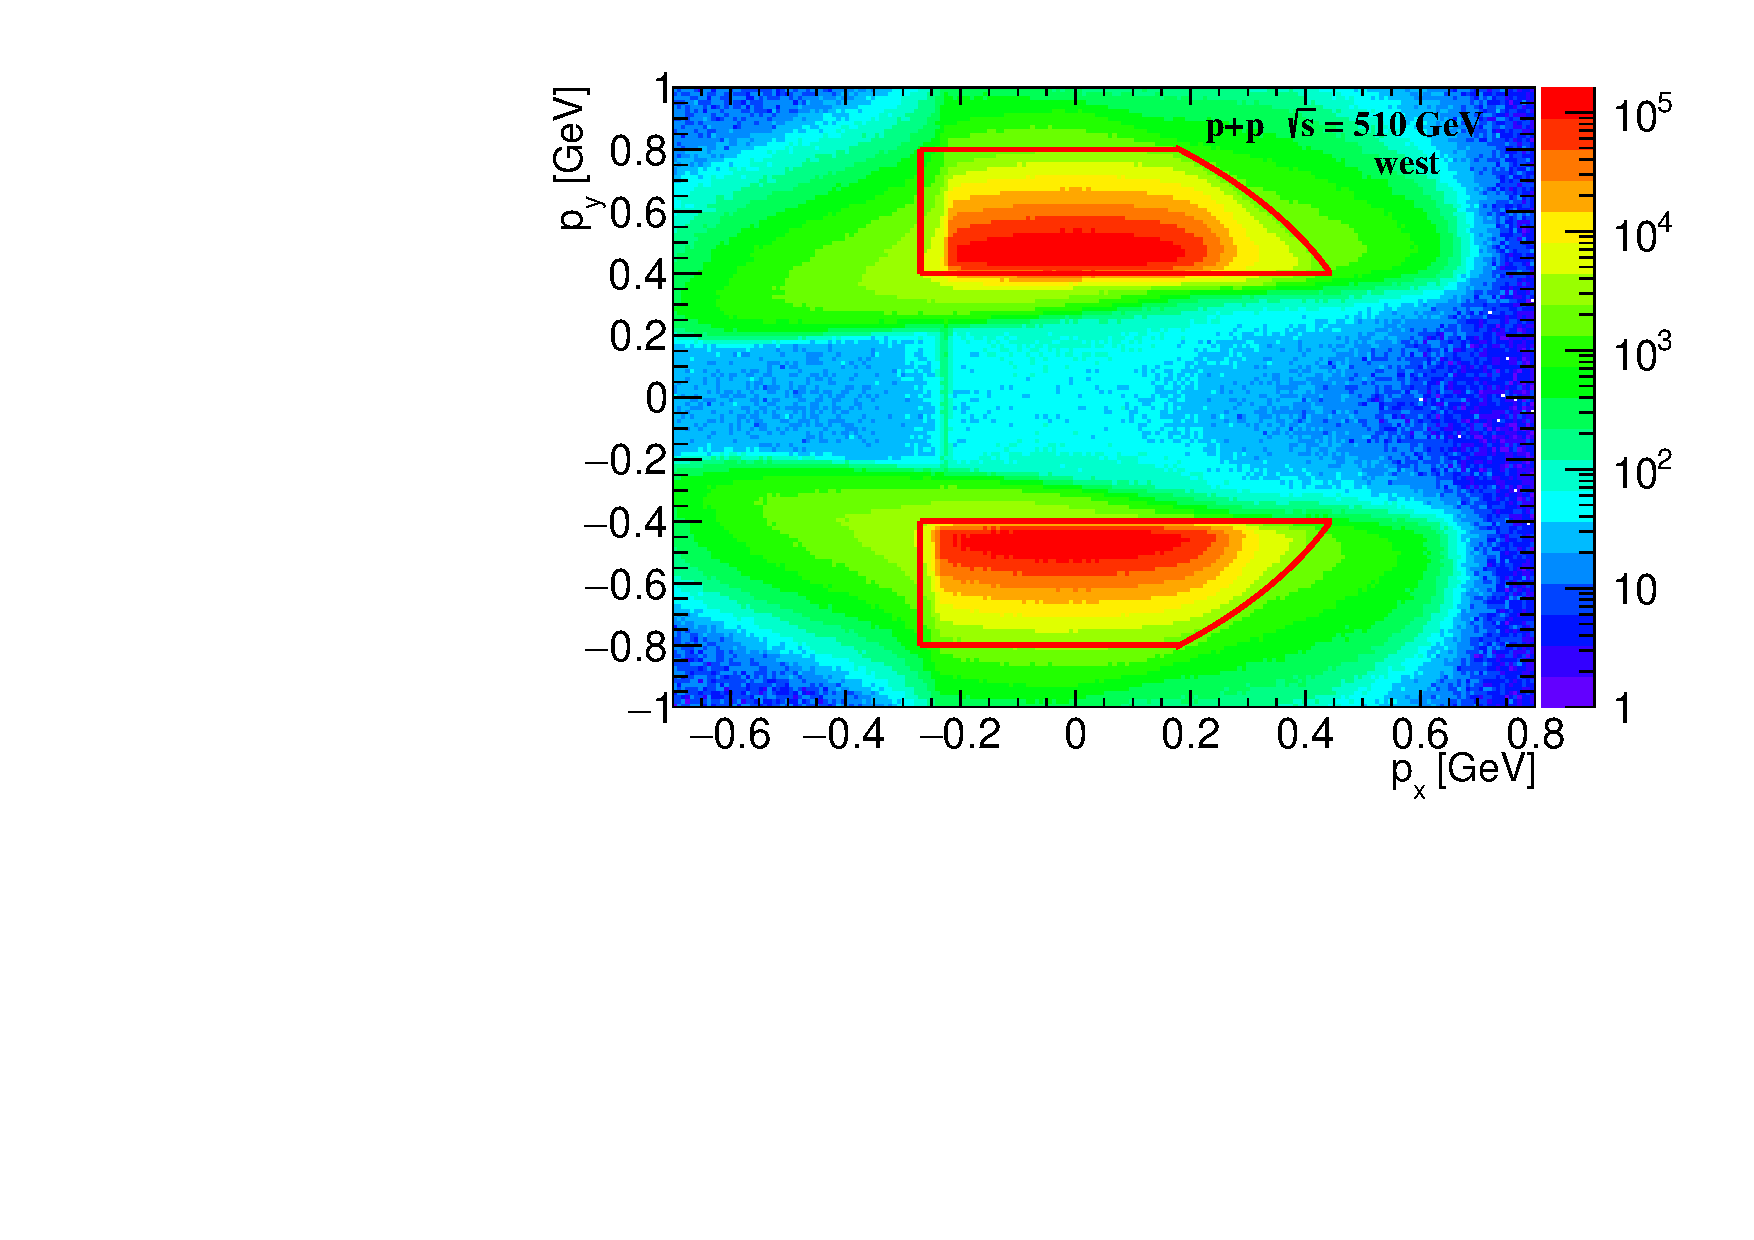
\includegraphics[width=1\textwidth]{figures/hRPcorrWest.pdf}
    \caption[Correlation graph of transverse momentum in Roman Pot system on the west side of the detector]{Correlation graph of transverse momentum in Roman Pot system on the west side of the detector.}
    \label{af4}
\end{figure}
\FloatBarrier

\FloatBarrier
\begin{figure}[ht]
    \centering
    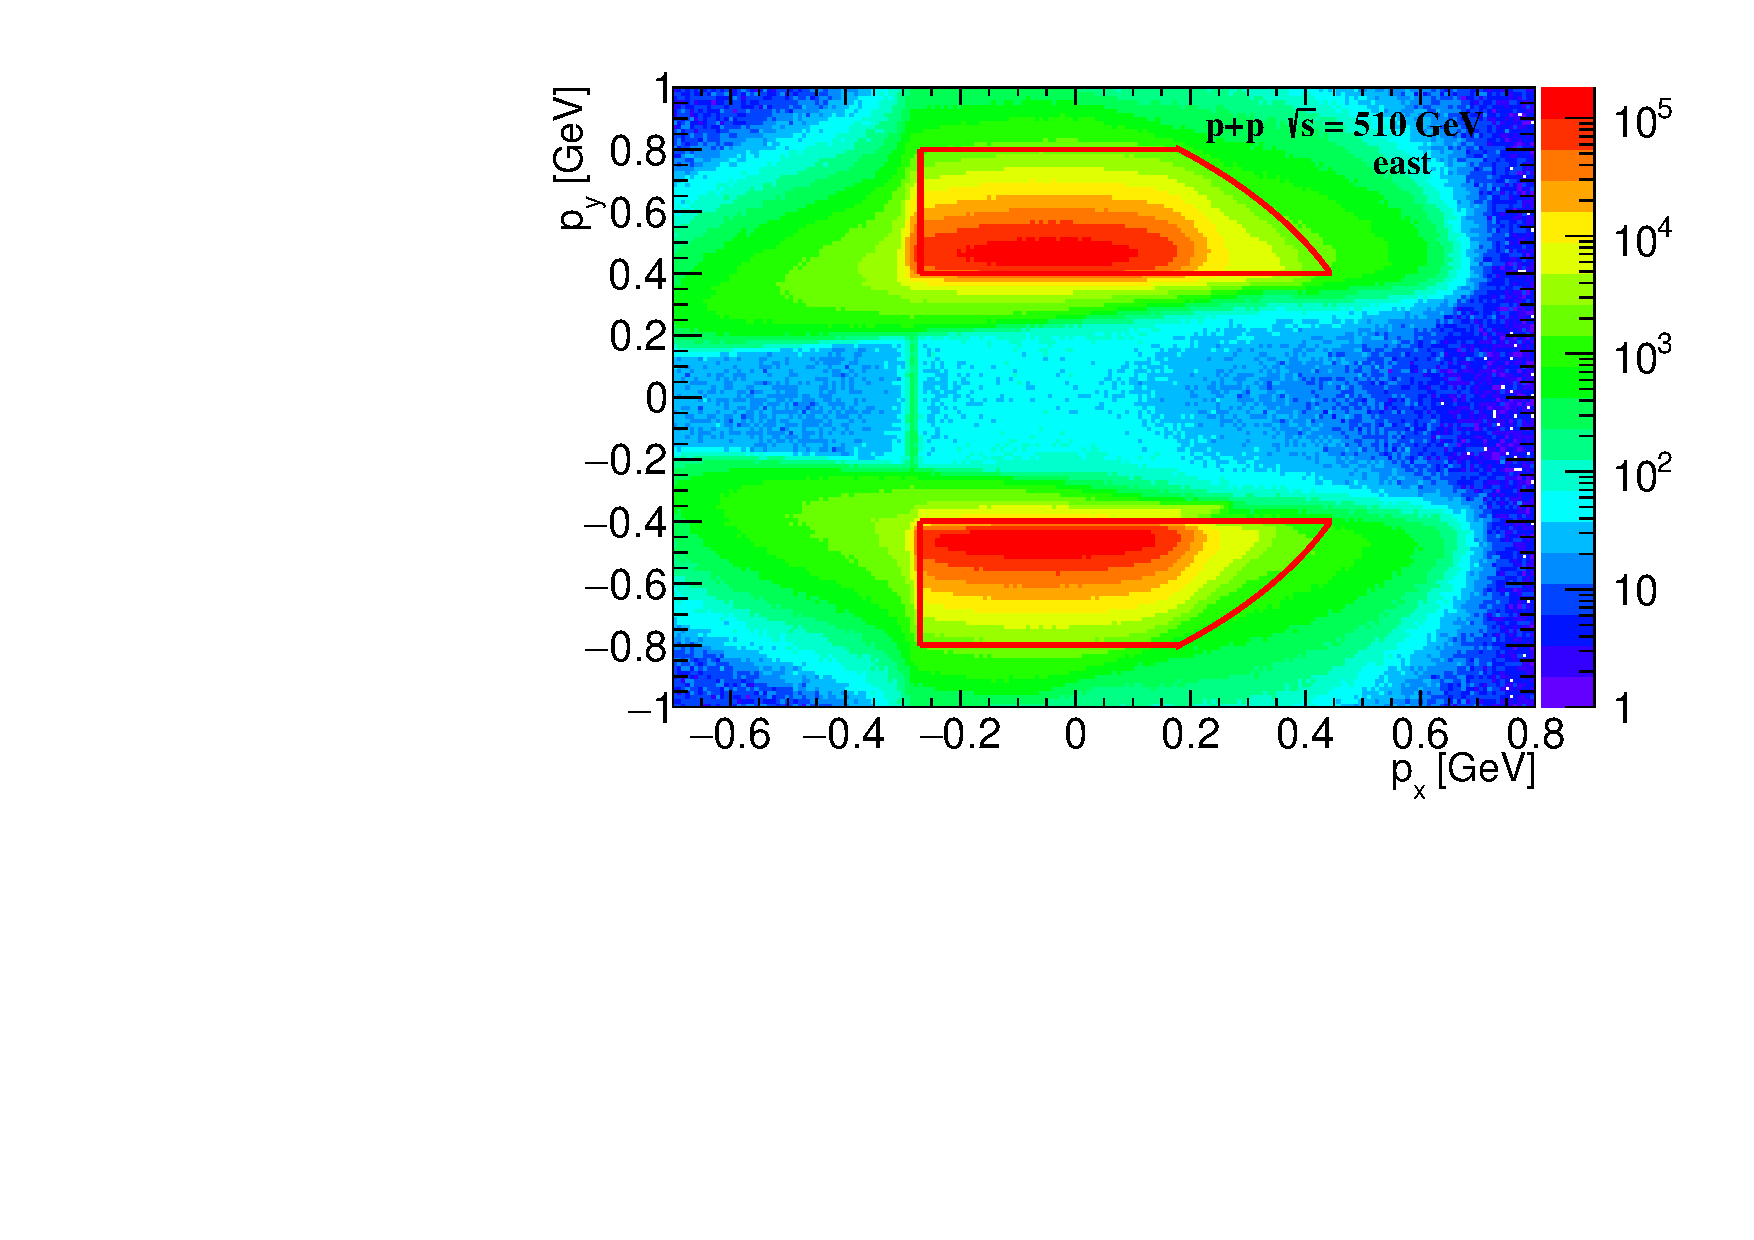
\includegraphics[width=1\textwidth]{figures/hRPcorrEast.pdf}
    \caption[Correlation graph of transverse momentum in Roman Pot system on the east side of the detector]{Correlation graph of transverse momentum in Roman Pot system on the east side of the detector.}
    \label{af17}
\end{figure}
\FloatBarrier
\subsection{Number of vertices}
\label{posZ}

\FloatBarrier
\begin{figure}[ht]
    \centering
    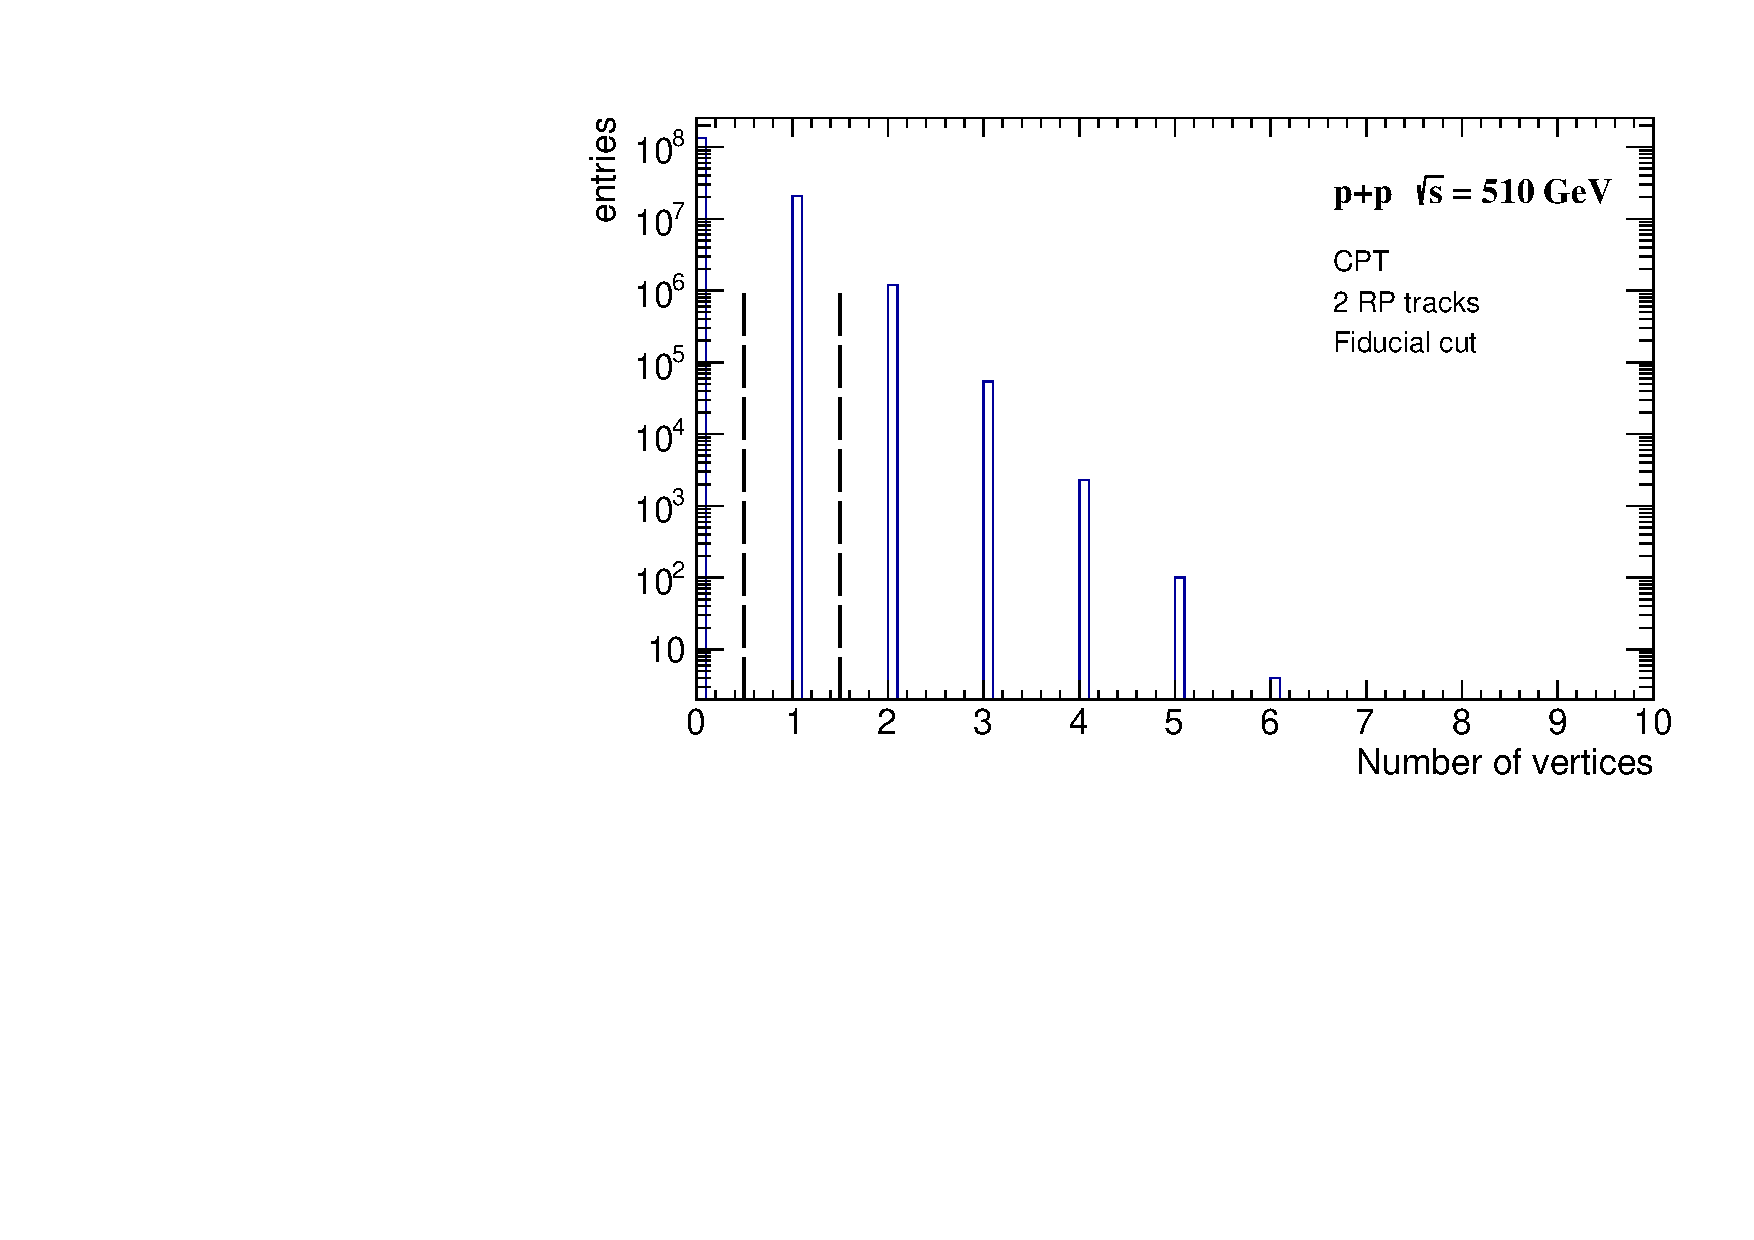
\includegraphics[width=1\textwidth]{figures/hNVertices.pdf}
    \caption[Distribution of number of vertices in the central tracking system]{Distribution of number of vertices in the central tracking system. The y coordinate is logarithmic scale.}
    \label{af69}
\end{figure}
\FloatBarrier

Moving on to central tracking system, the first condition is imposed on number of vertices. The condition is to have 1 and only 1 vertex. The position of vertex is reconstructed from the particle tracks in TPC. To be exact, the reconstructed vertex for the processes that are interesting for this thesis is not the primary but the secondary vertex of the event where the measured neutral particle decays into the hadron pair. The position of primary vertex is not known due to the small number of tracks. The primary vertex of the event would be located less than $3$ cm and $8$ cm away from the secondary vertex for $K^0_S$ and $\Lambda^0$ respectively\footnote{If we consider the PDG values \cite{zyla} for lifetimes to be $8.954 \pm 0.004$ $10^{-11}$ s ($K^0_S$) and $2.63 \pm 0.02$ $10^{-10}$ s ($\Lambda^0$) and that they move with the speed of light $c=2.999~792$ m/s, then the distance travelled will be around the previously mentioned values.}. The distribution of number of vertices can be seen in \autoref{af69}.
\subsection{Vertex position of z coordinate}
 Another condition regards the position of z coordinate of vertex. For an event to pass the condition, it's vertex has to satisfy $|z_{vertex}| < 80$ cm from the interaction point which is the absolute middle of the detector. The reason for this condition is to have the best acceptance, effectiveness and 
to minimize the systematic errors.
\FloatBarrier
\begin{figure}[ht]
    \centering
    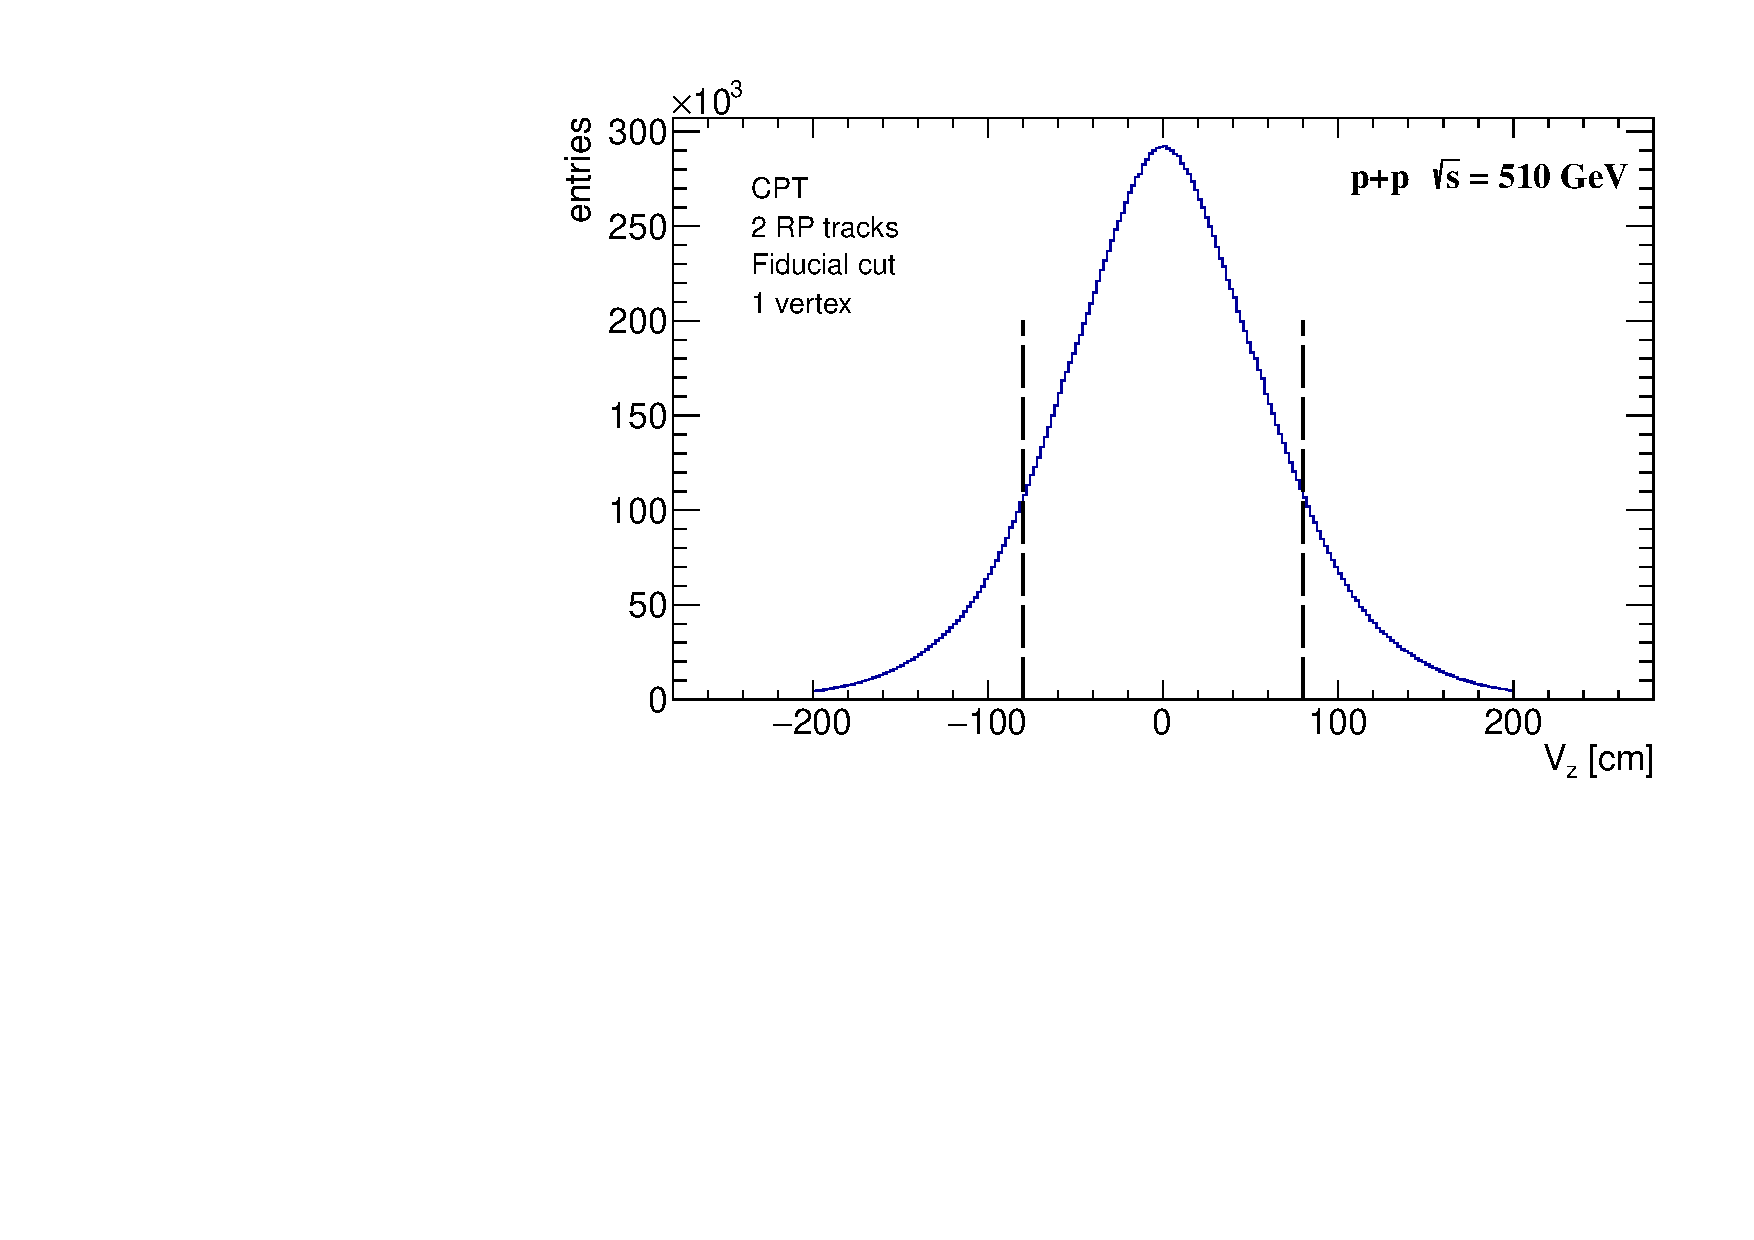
\includegraphics[width=1\textwidth]{figures/hPosZ.pdf}
    \caption[Distribution of z coordinate position of vertex]{The graph of distribution of z coordinate of vertex. Events that satisfy the condition $|z_{vertex}| < 80$ cm are selected.}
    \label{af5}
\end{figure}
\FloatBarrier
\subsection{2 tracks in TOF + other}
This next cut includes several conditions. The first condition is that only 2 hadron tracks per 1 event are allowed to be registered in the TOF detector. In addition, this condition allows studying exclusive events.
\newline
Another 2 conditions are based on the Distance of the Closest Approach (DCA) position. It is the distance between the closest point on the reconstructed track to the primary vertex. Because the position of the primary vertex of measured particles $K^0_S$ and $\Lambda^0$ is not known, the secondary vertex is assumed to be primary as it was mentioned in \autoref{posZ}. Framework \textit{upcDst} contains only primary tracks and not global, but the incorporation of global tracks is in progress. The conditions are separate for z coordinate and position in the transverse plane: $|DCA_z| < 1$ cm and $DCA_{xy} < 1.5$ cm and can be seen in \autoref{af6} and \autoref{af17}. 
\FloatBarrier
\begin{figure}[ht]
    \centering
    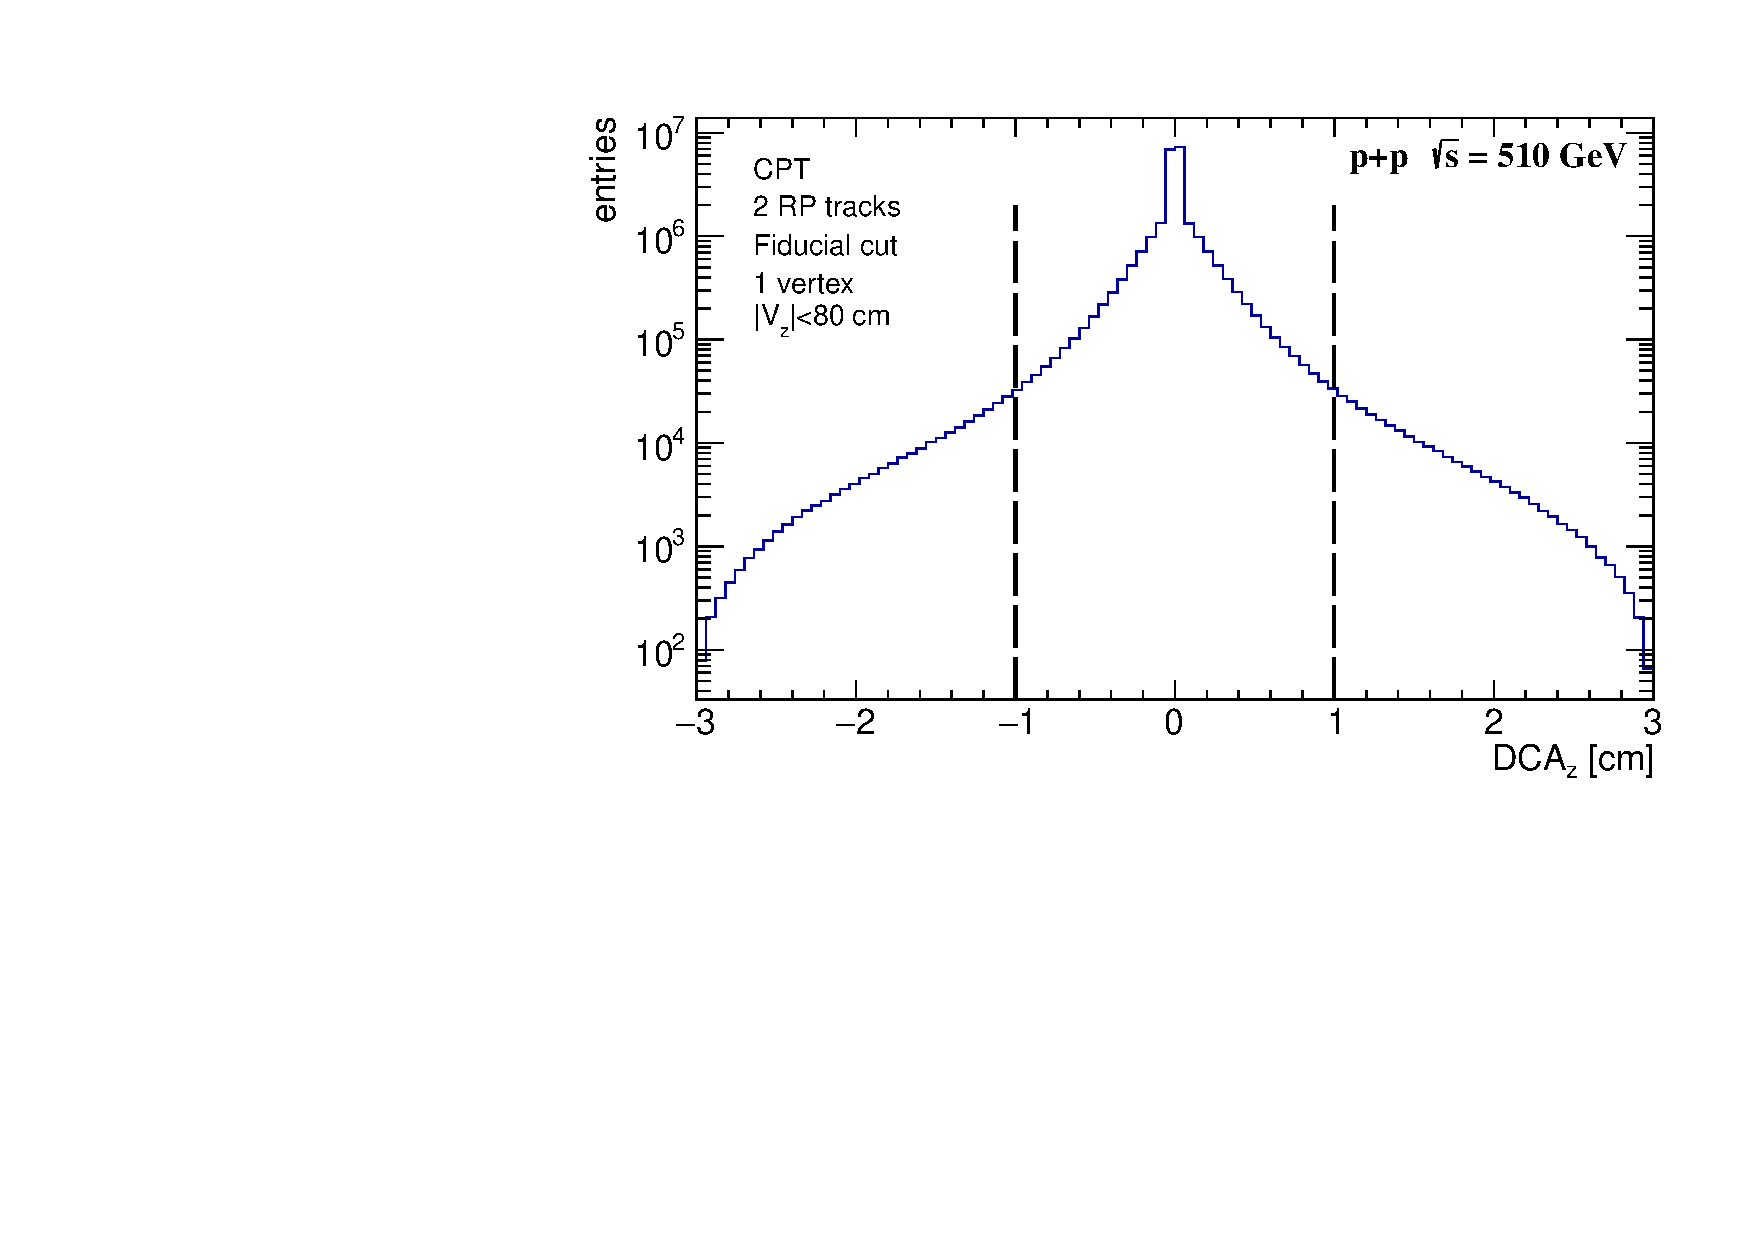
\includegraphics[width=1\textwidth]{figures/hDcaZ.pdf}
    \caption[Distribution of z coordinate of DCA]{Graph of distribution of DCA for z coordinate with logarithmic scale on vertical axis. The condition for z coordinate is $|DCA_z| < 1$ cm.}
    \label{af6}
\end{figure}
\FloatBarrier
\FloatBarrier
\begin{figure}[ht]
    \centering
    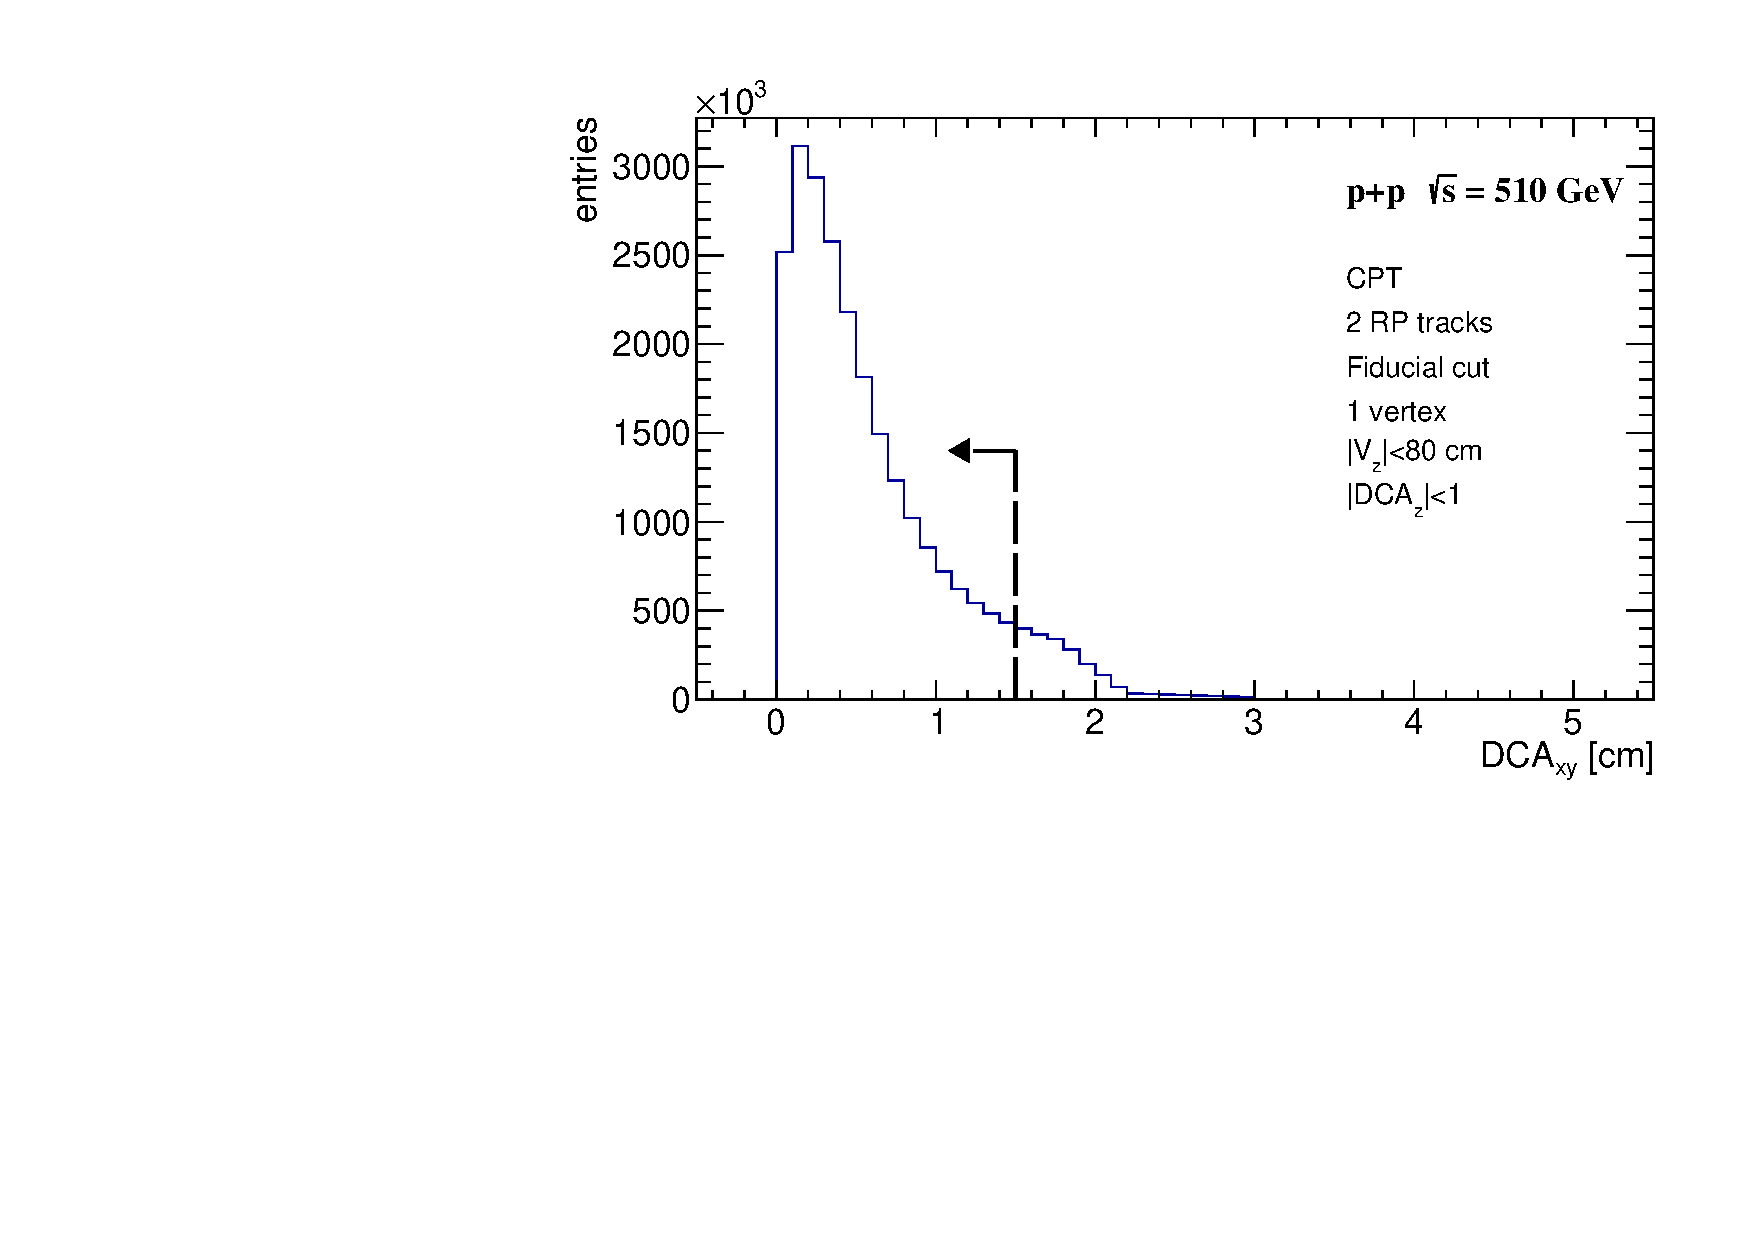
\includegraphics[width=1\textwidth]{figures/hDcaXY.pdf}
    \caption[Distribution of DCA $(x,y)$ plane] {Graph of distribution of DCA in the transverse plane $(x,y)$. Imposed condition is $DCA_{xy} < 1.5$ cm.}
    \label{af17}
\end{figure}
\FloatBarrier
Another 2 cuts are imposed on the number of hits in TPC. The bigger the number of hits is, the better is the resolution as it was described in \autoref{tpc}. For satisfactory track reconstruction and energy loss measurement numbers of hits 25 and 15 were required. Graphs for distributions can be seen in \autoref{af7} and \autoref{af16}. These are standard STAR conditions used at STAR.

\FloatBarrier
\begin{figure}[ht]
    \centering
    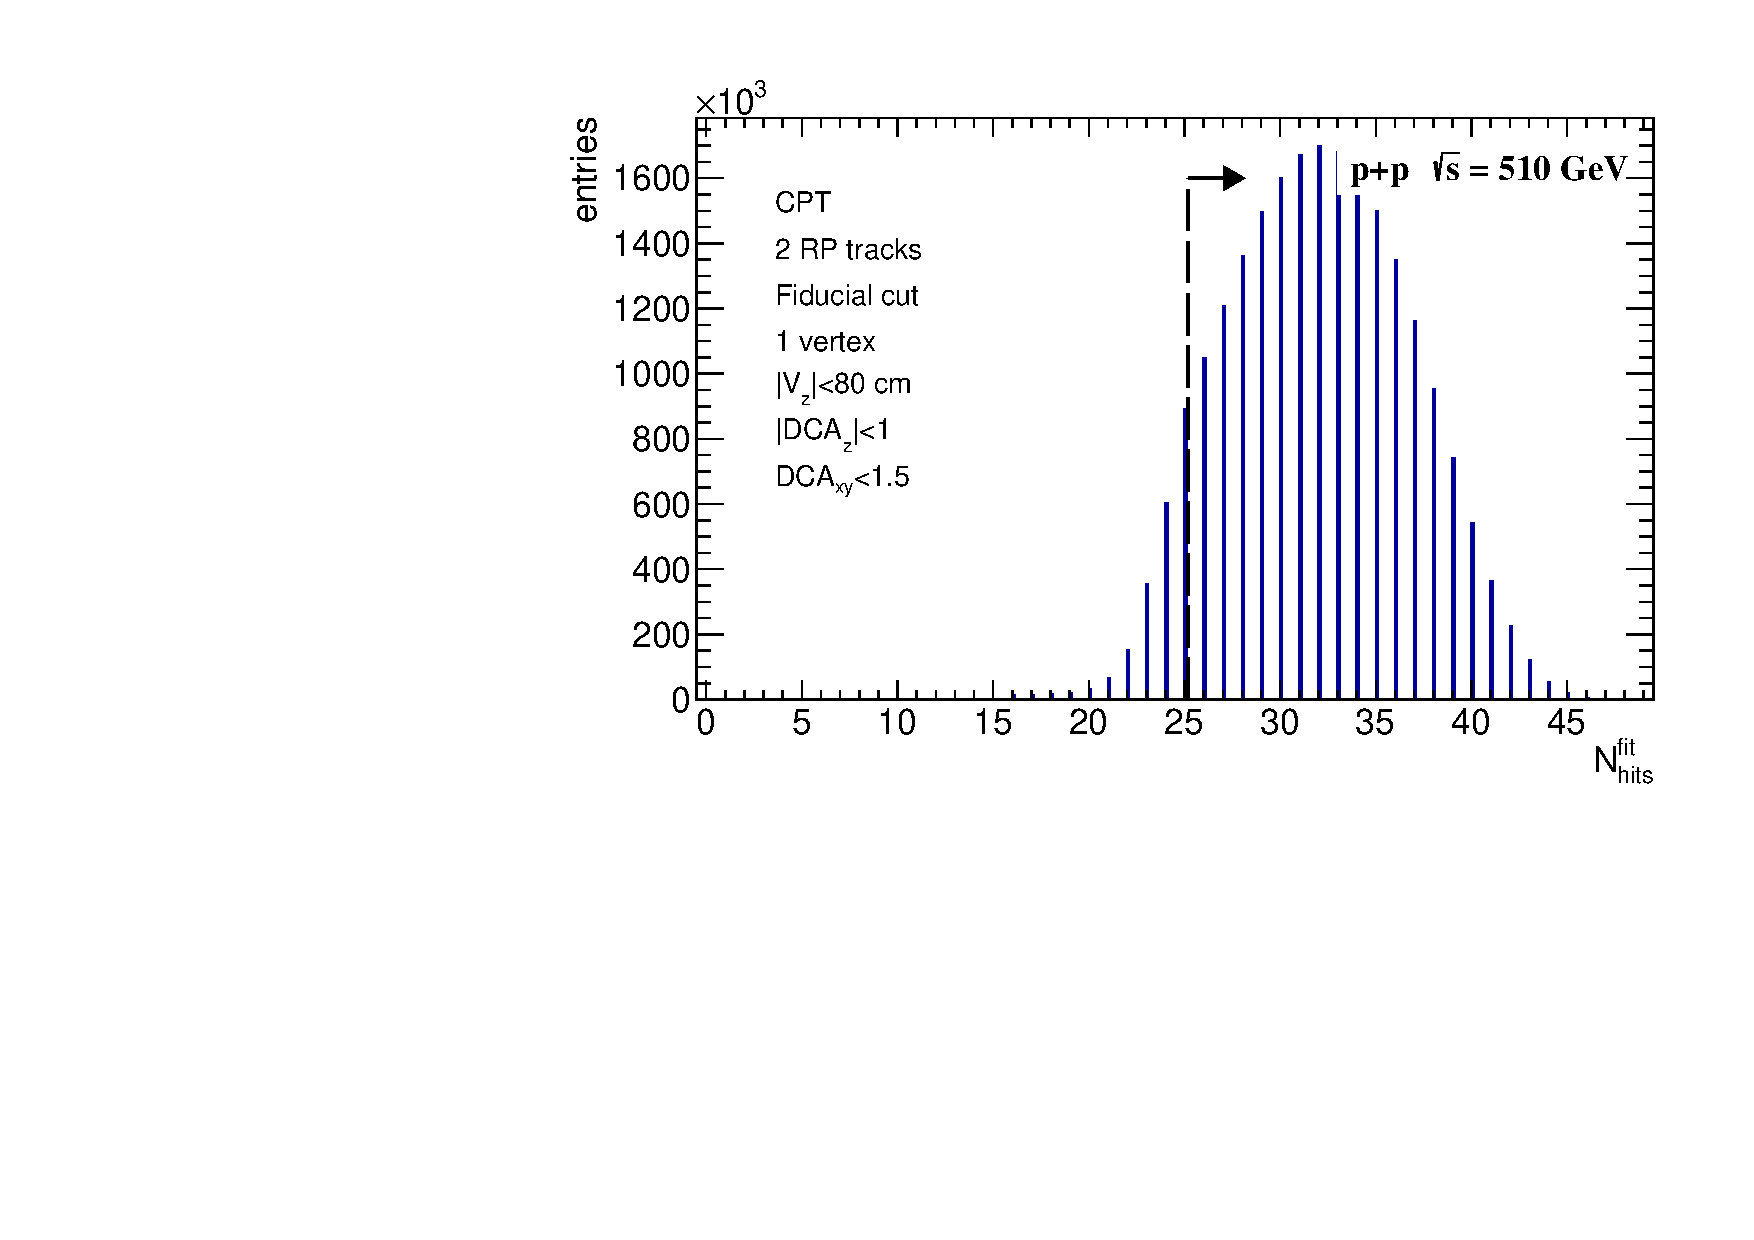
\includegraphics[width=1\textwidth]{figures/hNfitHits.pdf}
    \caption[Distribution of number of hits in TPC for track reconstruction]{Distribution of number of hits in TPC for track reconstruction.}
    \label{af7}
\end{figure}
\FloatBarrier

\FloatBarrier
\begin{figure}[ht]
    \centering
    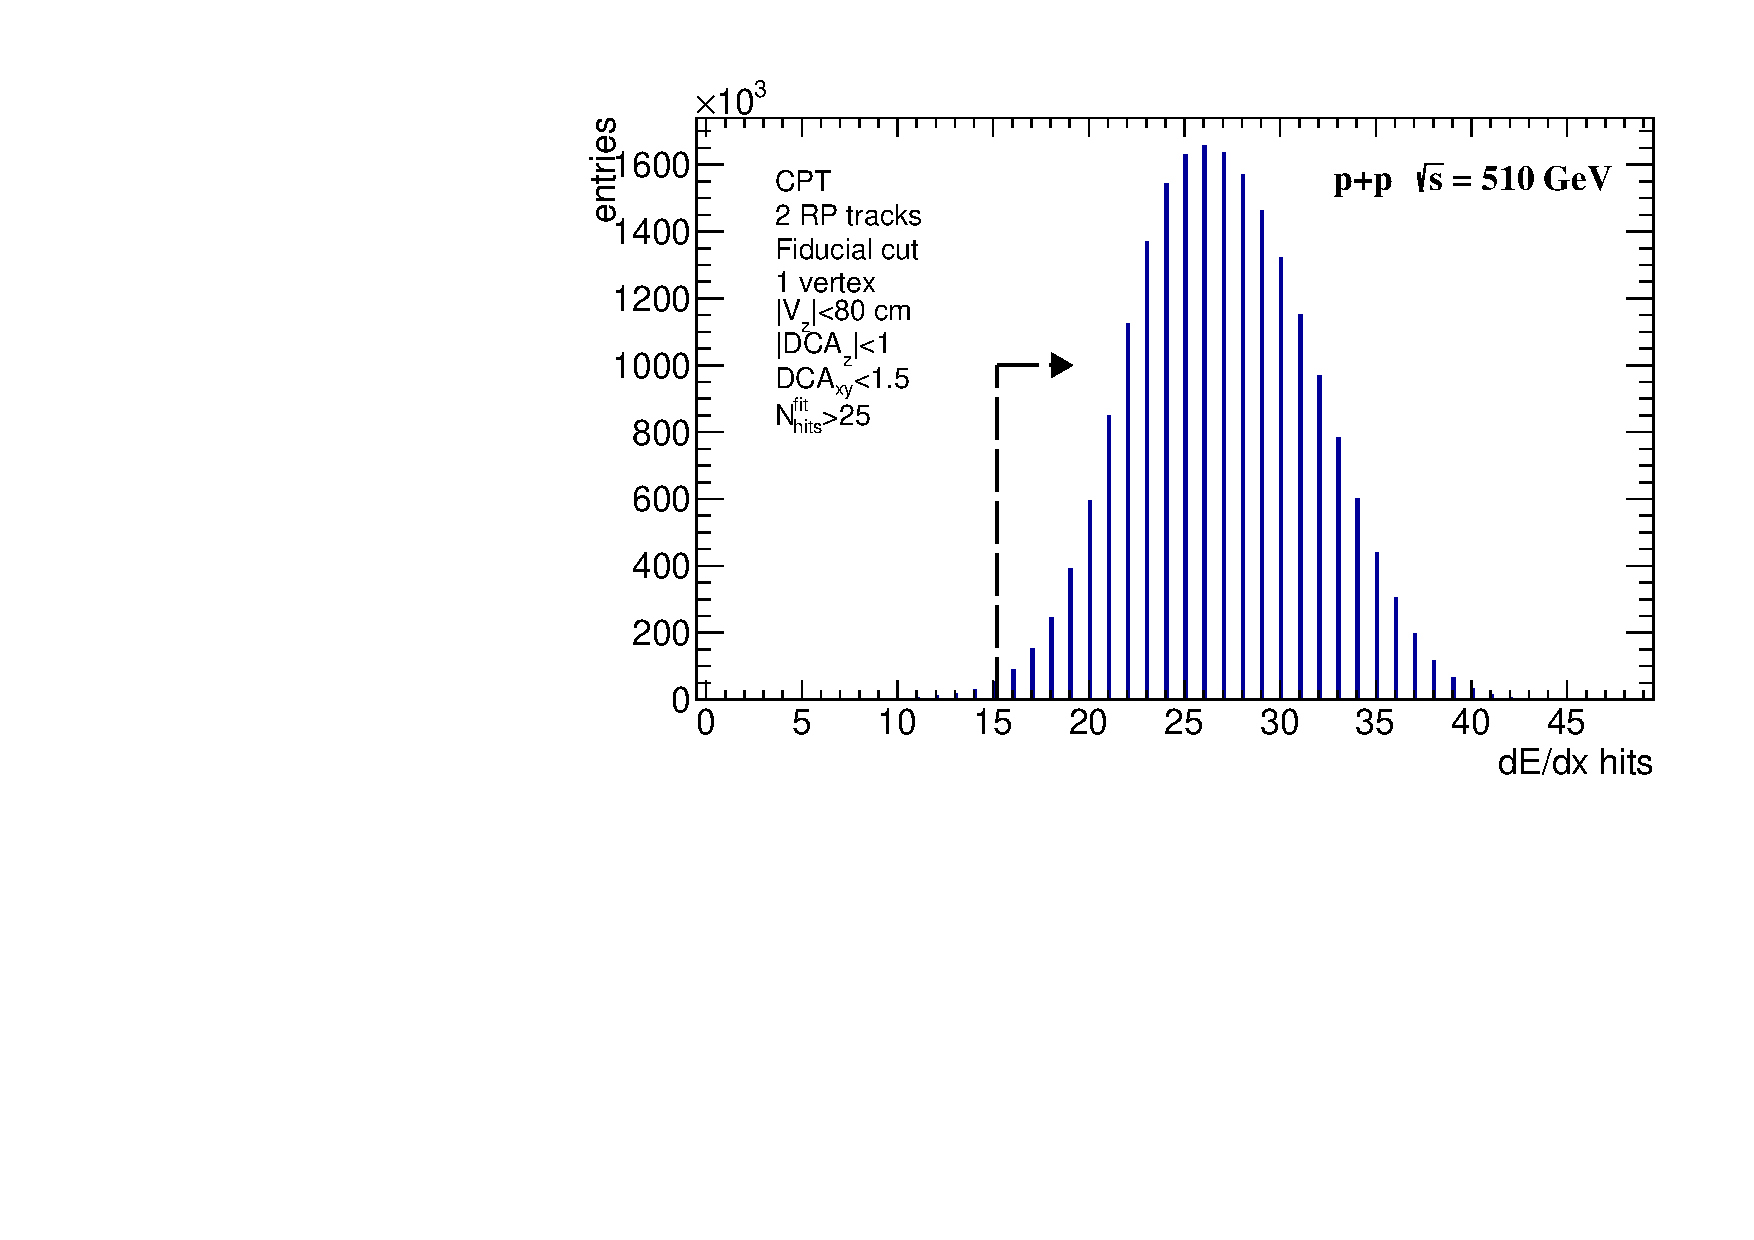
\includegraphics[width=1\textwidth]{figures/hNhitsDEdx.pdf}
    \caption[Distribution of number of hits in TPC for energy loss measurement]{Graph of distribution of number of hits for energy loss measurement.}
    \label{af16}
\end{figure}
\FloatBarrier

\subsection{Pseudorapidity}
The following condition considers the pseudorapidity of the scattered hadrons. Even though nowadays the acceptance of the TPC detector is quite high ($|\eta| < 1.5$) the measurement was done before the upgrade so the events chosen for the analysis have to satisfy the condition $|\eta|<0.7$. The reasoning behind this condition is that the hadrons have to be within the TOF acceptance. The pseudorapidity distribution and the imposed cuts can be seen in \autoref{af8}.

\FloatBarrier
\begin{figure}[ht]
    \centering
    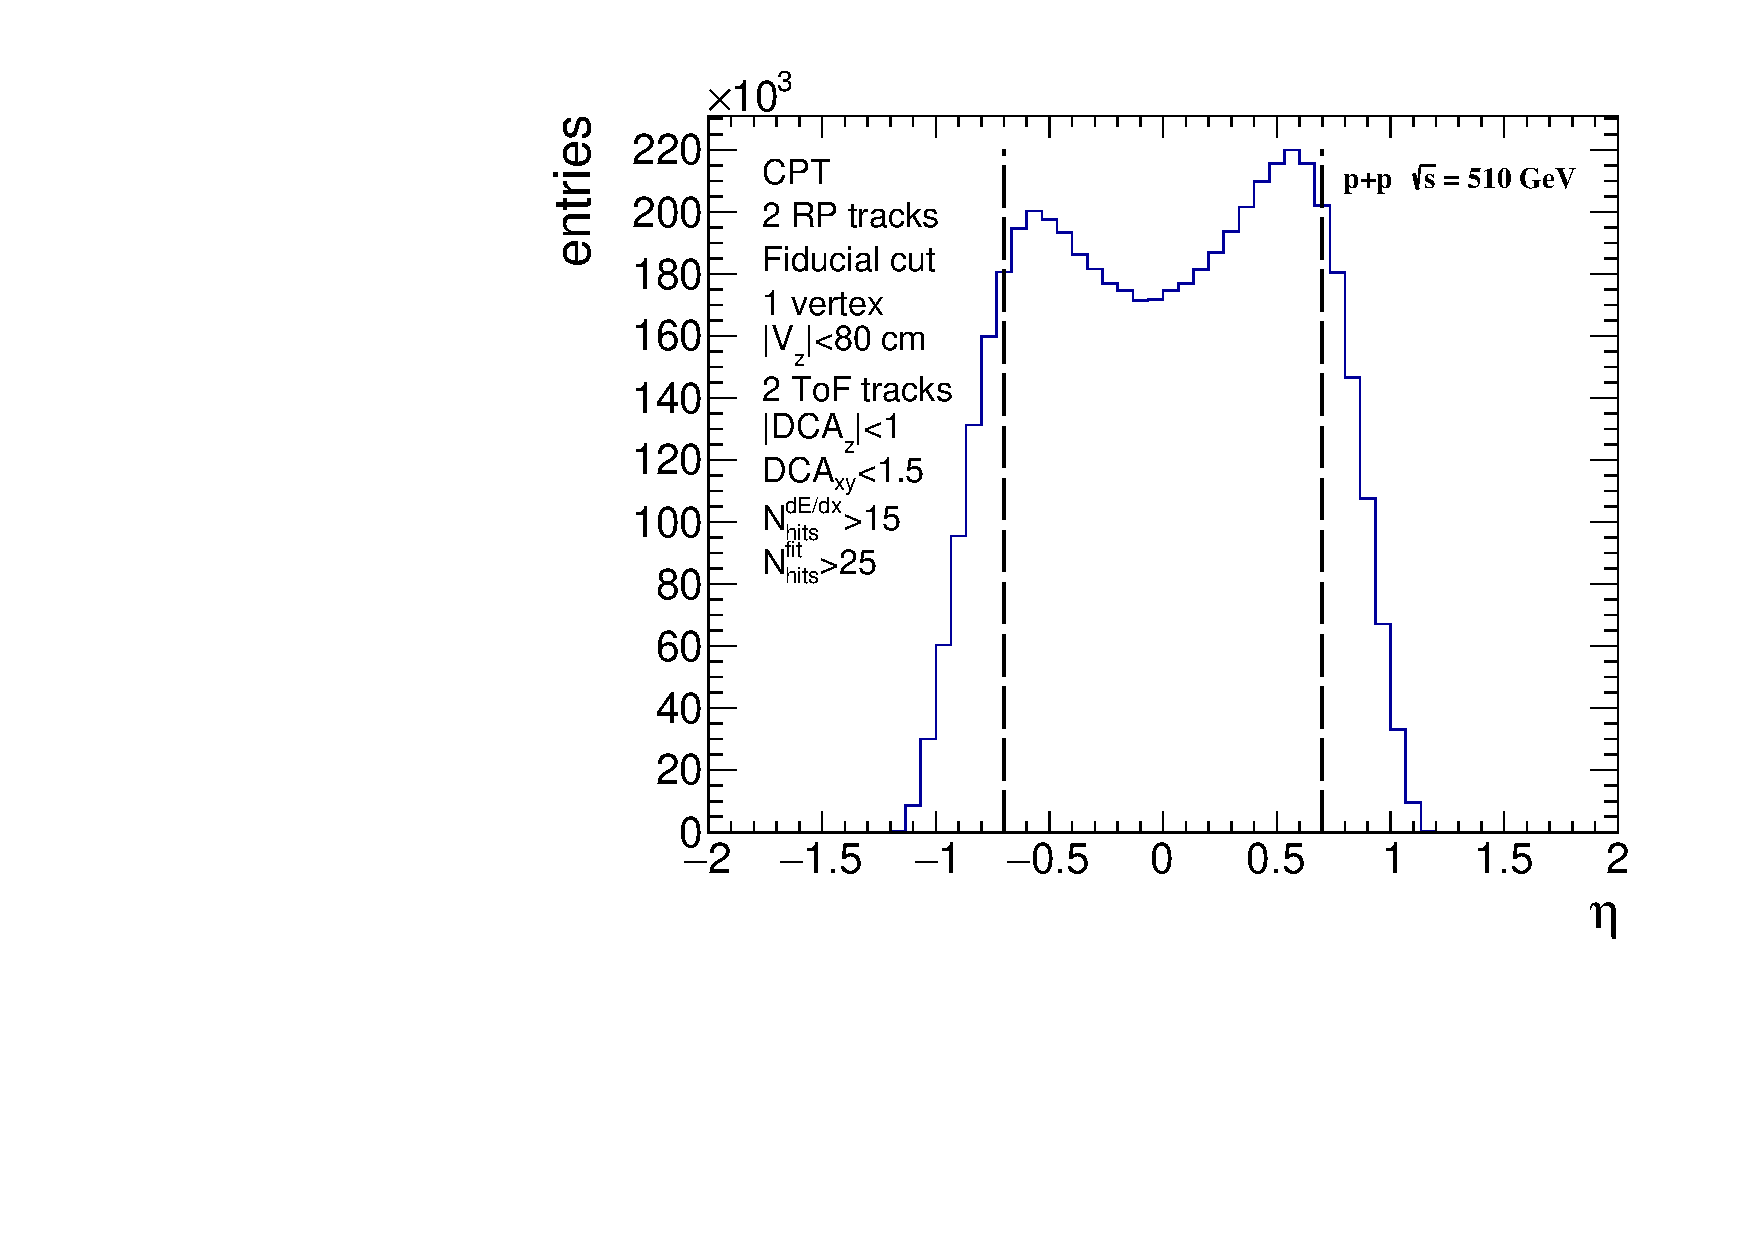
\includegraphics[width=1\textwidth]{figures/hEta.pdf}
    \caption[Distribution of pseudorapidity of measured hadrons]{Graph of distribution of pseudorapidity for created hadrons. The selected events must satisfy $|\eta| < 0.7$. }
    \label{af8}
\end{figure}
\FloatBarrier

\subsection{Total charge}
The last condition imposed on the selection of events is that the total charge of the created hadron pair has to be equal to 0\footnote{This condition comes in the analysis after particle identification to ensure the quality of the background.}. Based on the charge, pairs are divided into 2 categories: like-sign and unlike-sign pairs. Like sign pairs are considered as background and can be seen in invariant mass distributions in \autoref{resultS}.

\section{Particle identification}
This section debates the identification of particles and separates events based on their relevance. The relevant particle pairs are $\pi \pi$ and $p \pi$. As mentioned before, the charges will be regarded later.
\newline
Particle identification is based solely on the energy loss measurement from TPC which is plotted against the particle momentum. Distributions of particles that passed pseudorapidity cut can be seen in \autoref{af9}. The colored lines represent the expected value for different particles. Based on the measured particle's position on the graph, it is possible to determine which particle it is. That is done using the $n \sigma$ scale. Graphs that show the same dependence, only differ between the charges of identified particles, can be found in \autoref{appendixA}.
\FloatBarrier
\begin{figure}[ht]
    \centering
    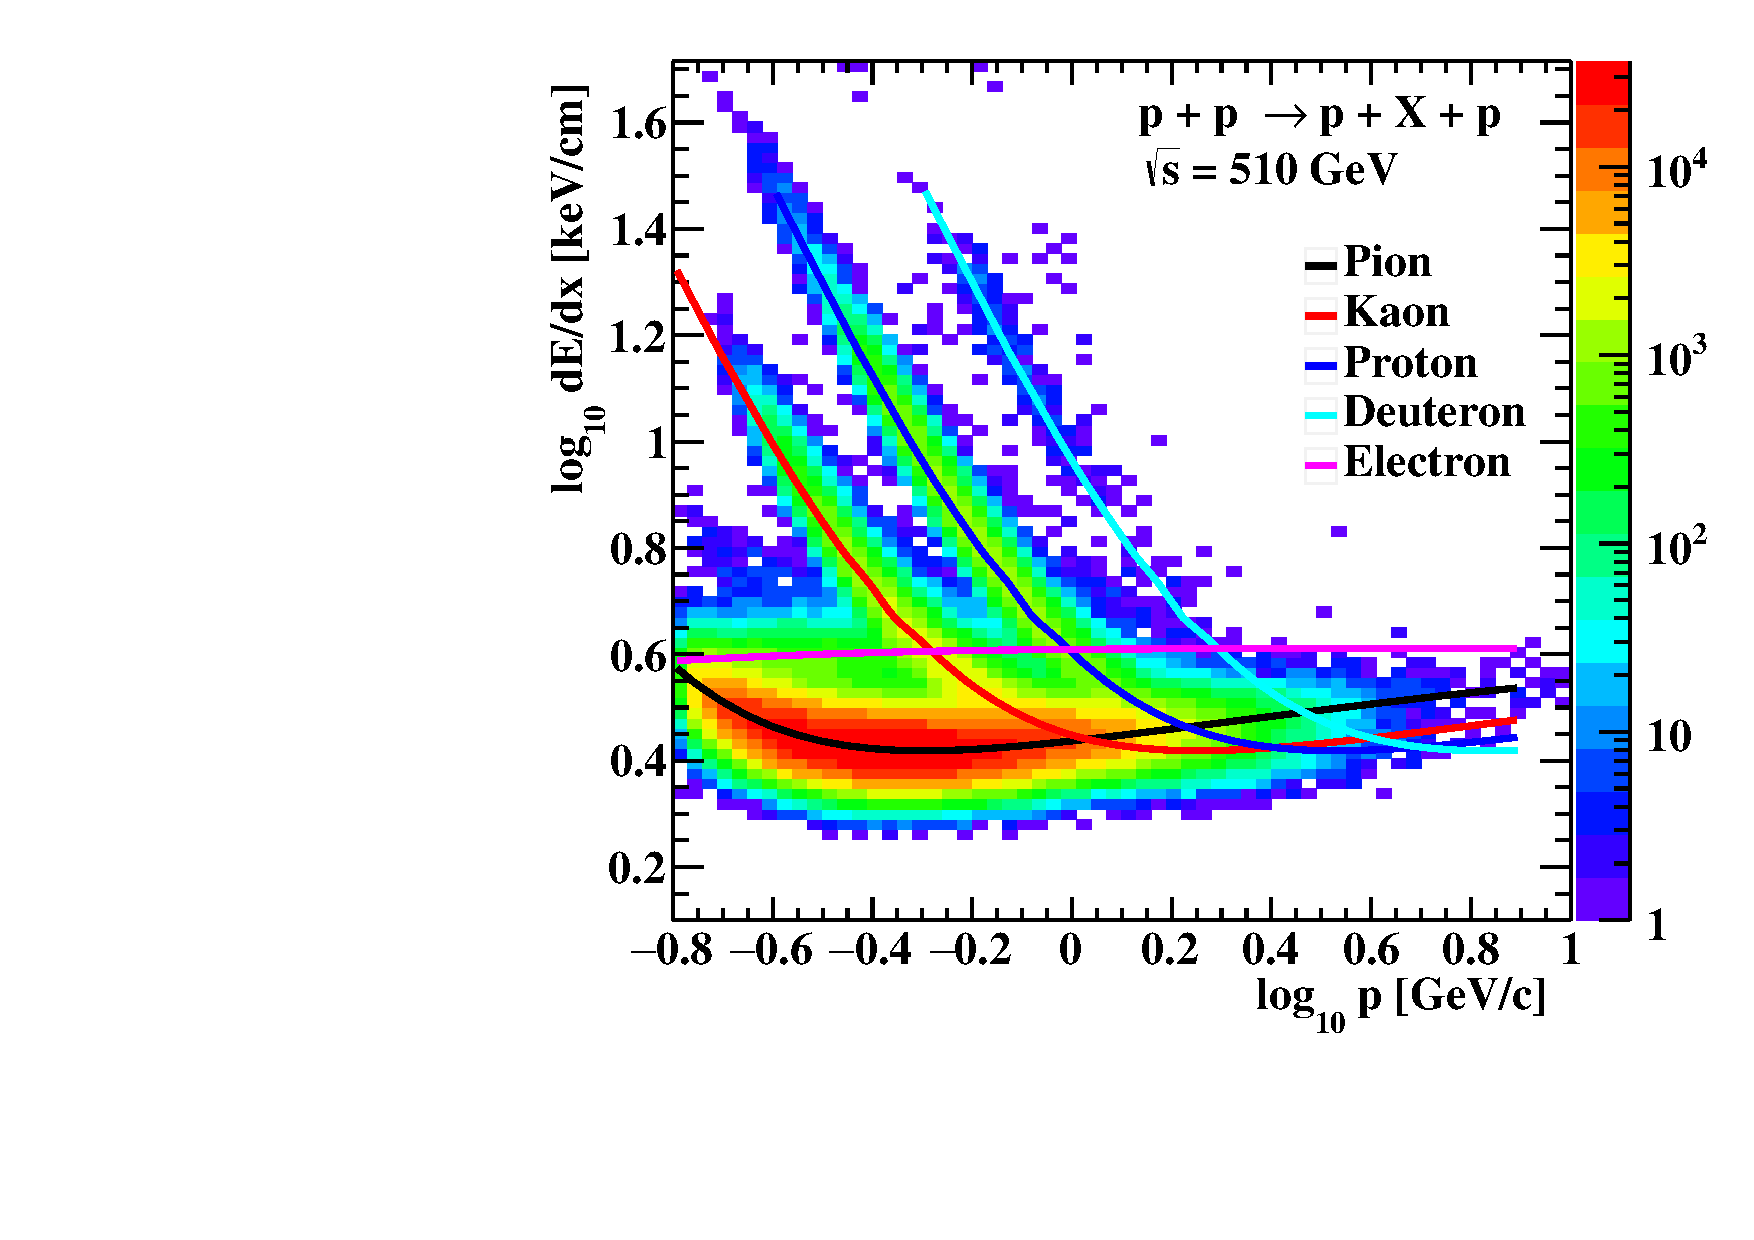
\includegraphics[width=1\textwidth]{figures/dEdx.pdf}
    \caption[Graph of hadron momentum and energy loss from TPC]{Correlation graph of hadron momentum and energy loss in keV/cm measured in TPC. All scales are logarithmic. }
    \label{af9}
\end{figure}
\FloatBarrier
\autoref{af9} shows that most of the particles that are measured by the TPC are pions, which are at the bottom of the graph and follow the black line. Next in line are kaons located around the red line followed by the protons positioned close to the blue line. The last line shown is the light blue line which represents deuterons. Even though the number of detected deuterons is negligible compared to number of other particles, there still are some. In \autoref{appendixA}, are shown the same graphs only they are divided based on the charge of particle. The graphs show that there are a few deuterons, but almost none antideuterons. Reason behind the detection of deuterons might be because of secondary interactions with particles in the beampipe.
\newline
The conditions for particle identification were as following,
\newline
\newline
\begin{minipage}{15cm}
\begin{myblock}{}
\centering
        $\textcolor{white}{\longrightarrow}if(n\sigma_{p}~<~3 ~~~\& ~~~n\sigma_{K}~>~3 ~~~\& ~~~n\sigma_{e}~>~3~~~ \& ~~~n\sigma_{\pi}~>~3)$
    \newline
    $\textcolor{white}{\longrightarrow}\textcolor{white}{\longrightarrow}$...
    \newline
        $\textcolor{white}{\longrightarrow}else~if(n\sigma_{p}~>~3 ~~~\& ~~~n\sigma_{K}~<~3 ~~~\& ~~~n\sigma_{e}~>~3~~~ \& ~~~n\sigma_{\pi}~>~3)$
    \newline
    $\textcolor{white}{\longrightarrow}\textcolor{white}{\longrightarrow}$...
    \newline
        $\textcolor{white}{\longrightarrow}else~if(n\sigma_{\pi}~<~3)$
    \newline
    $\textcolor{white}{\longrightarrow}\textcolor{white}{\longrightarrow}$...
\end{myblock}
\end{minipage}
\newline
\newline
First, protons were identified, on the grounds that the number of protons is the smallest (outside of deuterons which are irrelevant for this thesis). The condition imposed translates to particles being close enough to the proton line, but far enough from all the other lines. Same way were identified kaons. Lastly, pions are identified but they only have to satisfy the condition $n \sigma_{\pi}~<~3$. The reason for that is because pions are the majority of all particles and possible contamination with other particles is relatively low. Pions also hold a crucial role in the search for $K^0_S$ and $\Lambda^0$ and implementing a stronger condition might strongly affect the number of candidates for further analysis.
\FloatBarrier
\begin{figure}[ht]
    \centering
    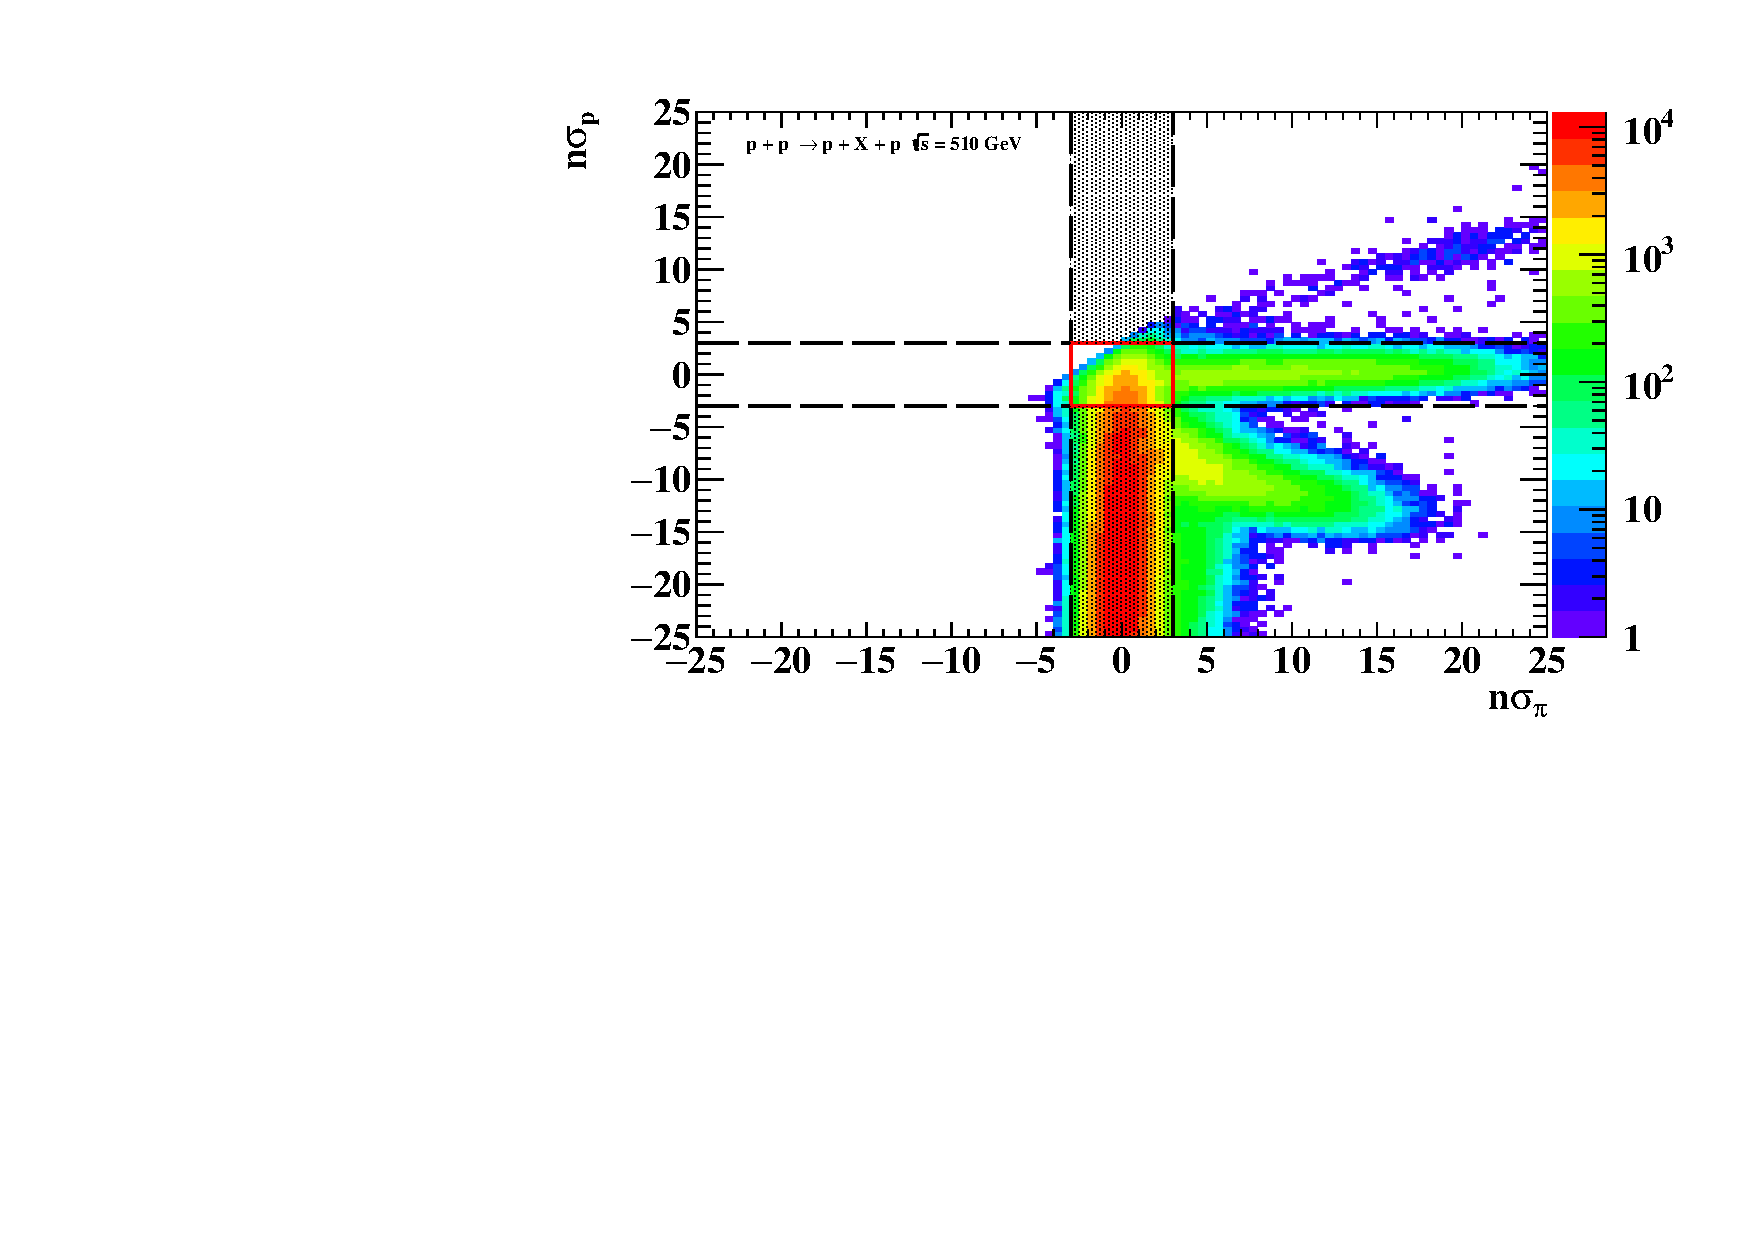
\includegraphics[width=1\textwidth]{figures/hNSigmaPiPcorr.pdf}
    \caption[Correlation graph of $n\sigma_{\pi}$ and $n\sigma_{p}$  of measured particles]{Correlation graph of $n_{\sigma}$ for pions on the x axis and $n_{\sigma}$ of protons on the y axis. Black lines represent the conditions for identification and the red box in the middle the overlay.}
    \label{af12}
\end{figure}
\FloatBarrier
\autoref{af12} is a correlation graph between $n \sigma$ for pions on the horizontal axis and protons on the vertical axis. Based on correlation plots for different particle pairs, which can be found in \autoref{appendixB}, particles on the right and parallel to pions in \autoref{af12} are electrons. Moving counter clockwise, the next band of particles represents kaons. Then follow protons and in last position are deuterons. 
